\chapter{Evaluation} \label{ch:eval}
Um das Konzept zu evaluieren, wird ein Prototyp nachgebaut.
Dieser wird in \autoref{ch6:prototype} erläutert.

In \autoref{ch6:bgs} werden zuerst die Definitionen zur Evaluation von \ac{BGS} vorgestellt, anhand deren die \ac{ROI}-Suche optimiert wird.
In \autoref{ch6:classifier} werden die Erhebung der Trainingsdaten für das \ac{CNN} und entsprechende Metriken vorgestellt.
Auf den Trainingsdaten werden mehrere \acp{CNN} trainiert und evaluiert.

In \autoref{ch6:inference} wird das Zusammenspiel beider Komponenten evaluiert, um einen Eindruck für die tatsächliche Performanz zu erhalten.

Zum Schluss wird in \autoref{ch6:scale} die notwendige Objektgröße untersucht.
Die Ergebnisse werden im Anschluss in \autoref{ch6:discussion} hinsichtlich der Anforderungen und Forschungsfragen diskutiert.


\section{Aufbau des Prototypen und Erstellen der Bildsequenzen} \label{ch6:prototype}
\label{ch4:masstab}
Der beschriebene Anwendungsfall wird im Maßstab $1:100$ nachgebaut:

\begin{itemize}
    \item Aus dem \SI{300}{\metre} Acker werden zwei \SI{3}{\metre} lange Teppiche in braun und grün, um eine höhere Diversität der Hintergründe zu gewährleisten.

    \item Die \SI{5}{\metre} langen Traktoren werden durch mehrere \SI{5}{\centi\metre} Modelle abgebildet; zusätzlich mehrere Varianten von Anhängern und Mini-LEDs, die als Scheinwerfer bei Nacht dienen.
    % Als Motor der Traktoren werden Nylonfäden eingesetzt, mit denen die Traktoren über das Feld gezogen werden.

    \item Die Kamera wird anstatt in \SI{100}{\metre} Höhe auf einem \SI{1}{\metre} hohem Stativ angebracht und Modellbäume stellen typische \IT{Störungen} da.
\end{itemize}

Inspiriert von den Ergebnissen üblicher Objekt Detektoren wurde initial eine Objektgröße von mindestens $32 \times 32$ Pixel angestrebt.
Zur Aufnahme der Bildsequenzen wurde daher der 8 Megapixel \SC{IMX179} Sensor von \SC{Sony} verwendet.
Damit entstanden $3264 \times 2448$ Pixel große Bilder.
Allerdings ergibt der Sensor bei maximalem Öffnungswinkel ein unscharfes Bild.
Für den Prototypen wurden jedoch scharfe Bilder präferiert, bei denen folglich die Objekte größer erscheinen.

Bei den Aufnahmen selbst wurde auf folgende Punkte Wert gelegt:
\vspace{-0.3em}
\begin{itemize}
    \setlength\itemsep{-0.1em}
    \item Unterschiedliche Fahrspuren der Traktoren
    \item Unterschiedliche Belichtungen bzw. Tageszeiten
    \item Unterschiedliche Traktor-Anhänger Kombinationen
    \item Unterschiedliche Fahrgeschwindigkeiten
    \item Teileweise Verdeckungen der Traktoren
    \item Tiere, die andere \IT{Bewegungen} darstellen
\end{itemize}

Um die Anforderungen an das System zu testen, werden die Wettereinwirkungen Nebel und Regen mit den Bibliotheken \SC{imgaug} und \SC{Automold} simuliert \cite{jung_imgaug_2019, ujjwal_automold_2019}.
Auf die Simulation von Schnee wurde verzichtet, da der Rotmilan zu dieser Jahreszeit nicht aktiv ist (siehe \autoref{ch1:motivation}).

\section{Background Subtraction} \label{ch6:bgs}
Der \ac{BGS} soll möglichst alle sich bewegenden Traktoren finden.
Um das zu testen, werden diese Traktoren händisch markiert\footnote{Zum Annotieren wurde \SC{LabelImg} verwendet \cite{tzutalin_labelimg_2020}}.
Eine Markierung besteht dabei aus Klasse und Boundingbox, die den Traktor einrahmt (siehe \autoref{ch2:fig:cv_problems}).
Aus dieser annotierten Boundingbox und den gefundenen \acp{ROI} des \ac{BGS} werden die \acp{IoU} gebildet.
Die Berechnung der \ac{IoU} wird in \autoref{ch6:iou} gezeigt.
Haben zwei Boxen eine mindest-\ac{IoU}, werden diese als Übereinstimmung gewertet und der Traktor ist somit gefunden.

In \autoref{ch6:bgs_opti} wird die Bestimmung der Parameter des \ac{BGS}s beschrieben, sodass mehr solcher Übereinstimmung gefunden werden.

\subsection{Definition: Intersection Over Union} \label{ch6:iou}
Die \ac{IoU} gibt das Verhältnis zwischen Schnittmenge (Intersection) und Vereinigung (Union) zweier Bereiche an.
Die \ac{IoU} wird dabei aus tatsächlicher Bounding Box $B_{gt}$ und vorhergesagter Bounding Box $B_p$ berechnet:
\begin{flalign}
    IoU &= \frac{area(B_p \cap B_{gt})}{area(B_p \cup B_{gt})}
\end{flalign}

Visualisiert sieht die \ac{IoU} zwischen $B_{gt}$ und $B_p$ wie in \autoref{fig:ch6:iou} aus.
\begin{figure}[ht]
    \center
    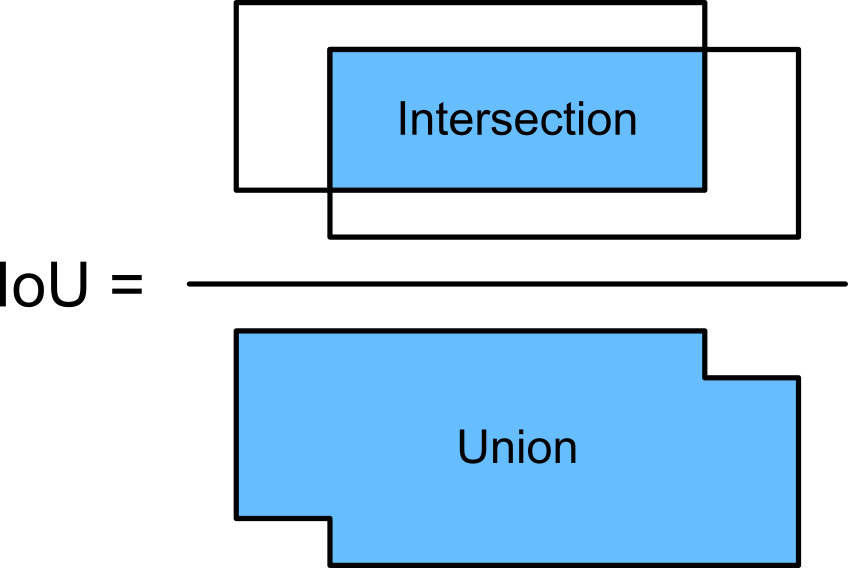
\includegraphics[width=0.5\textwidth]{figures/chapter_6/iou}
    \caption{Visualisierung der IoU zweier Bounding Boxen}
    \label{fig:ch6:iou}
\end{figure}

Die \ac{IoU} liegt zwischen $[0,1]$.
Eine \ac{IoU} von $0$ gibt an, dass die zwei Bereiche nicht überlappen und eine \ac{IoU} von $1$, dass es sich um identische Bereiche handelt.

\subsection{Vorgehen bei der Optimierung} \label{ch6:bgs_opti}
Für die Tests werden zwei Sequenzen (Tag und Nacht) annotiert.
Anschließend werden für die originalen und augmentierten (Nebel und Regen) Bildsequenzen alle \acp{ROI} gesucht und verglichen.

Zum Testen der Übereinstimmung wurde für die Tagsequenzen eine \ac{IoU} von $0.4$ und für die Nachtsequenzen eine \ac{IoU} von $0.3$ gewählt.
Das hat den Grund, dass bei den Nachtsequenzen vom \ac{BGS} oft nicht der annotierte Traktor gefunden wird, sondern nur Licht oder Lichtkegel.
Das ist beispielhaft in \autoref{apx:bgs_iou} zu sehen.

\bigskip
Für den Anfang wurden für \ac{BMOG} die gleichen Parameter wie für den \ac{CDW} Wettbewerb verwendet und für die Blobanalyse eine Mindestgröße von $32 \times 32$ Pixeln.
Dabei wurden sehr viele Traktoren bei Nacht nicht gefunden (vgl. \autoref{fig:ch6:bgs_start}).
Ebenfalls wurden insgesamt nur sehr wenige \acp{ROI} für die Nachtsequenzen vorhersagt.
Es gilt daher die gleiche Annahme wie für die kleinere \ac{IoU}: nur das Licht wird gefunden, welches nur einen kleinen Teil des Traktors darstellt.

\begin{figure}[ht]
    \begin{small}
        \begin{center}
            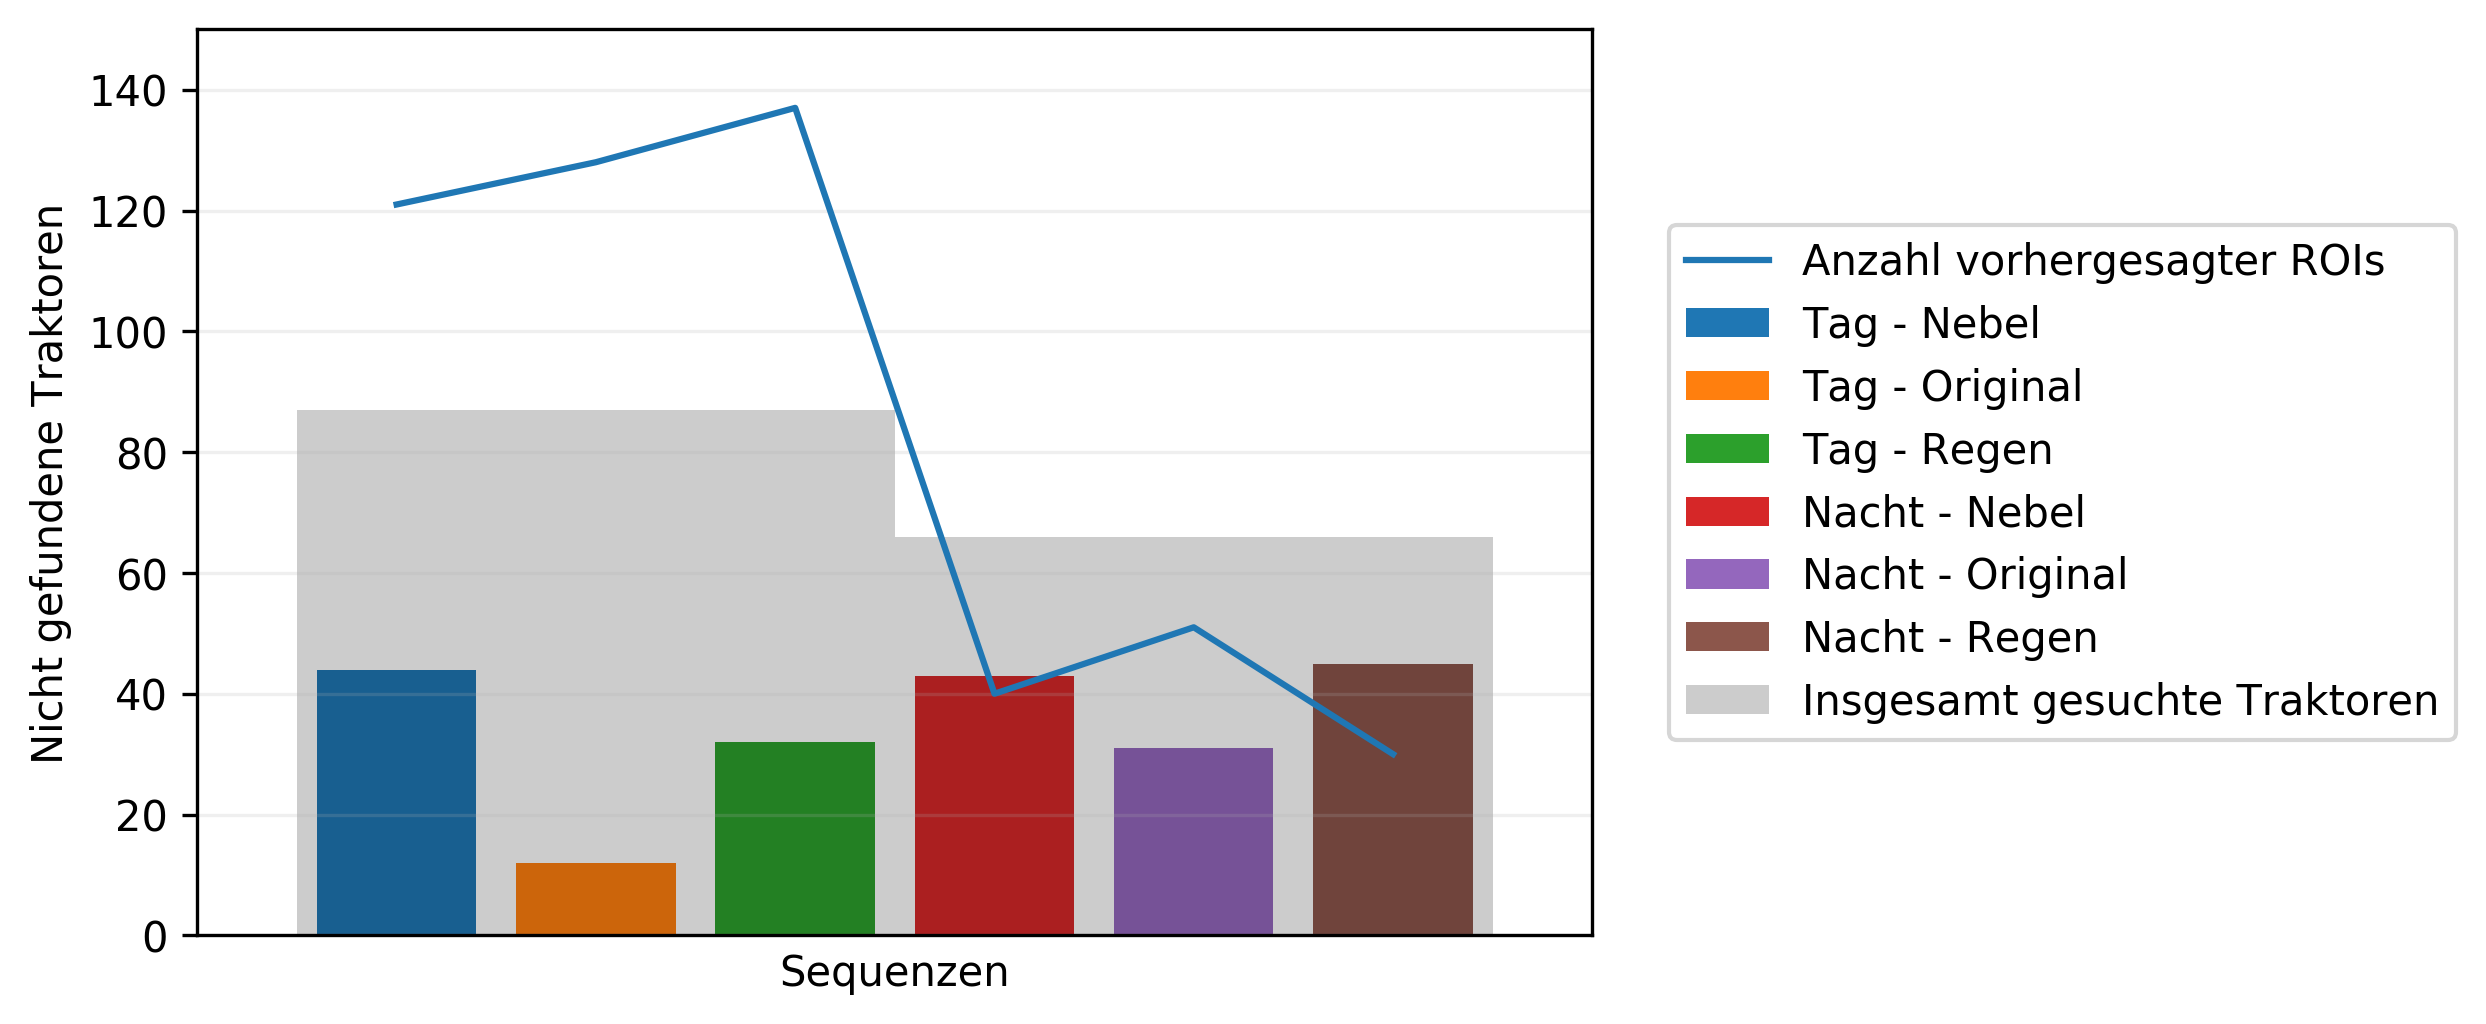
\includegraphics[width=0.95\textwidth]{figures/chapter_6/bgs-start}
        \end{center}
        \caption[Ergebnisse für BGS mit Startkonfiguration]
        {\BF{Ergebnisse für \ac{BGS} mit Startkonfiguration.}
        Beschreibung des Plots:
        \begin{itemize*}
            \item die farbigen Balken repräsentieren die nicht gefundenen Traktoren der jeweiligen Sequenz (je niedriger, desto besser)
            \item die grauen Balken geben die gesuchten Traktoren an
            \item die blaue Linie gibt die jeweils vom \ac{BGS} gefundenen \acp{ROI} an (je weniger, desto besser)
        \end{itemize*}}
        \label{fig:ch6:bgs_start}
    \end{small}
\end{figure}

Die Mindestgröße für die Blobanalyse wurde deshalb auf $15$ Pixel reduziert.
Dadurch stieg allerdings die Anzahl der Vorhersagen für die Regensequenzen stark an.

Um dem vielen Rauschen der Regensequenzen entgegenzuwirken, wurde der \ac{BMOG} interne Parameter \SC{Postprocessing} von $9$ auf $15$ erhöht.
Dadurch wird die Vordergrundmaske stärker weichgezeichnet, sodass die Regentropfen verwischt und so herausgefiltert werden.

Bei Betrachtung der Vordergrundmaske fiel ferner auf, dass die Vordergrundobjekte nur knapp nicht \IT{zusammenwuchsen} und ein Objekt somit als zwei interpretiert wurde.
Daher wurde die morphologische Dilatation $15$-fach angewandt, bei der die Objekte ausgedehnt werden und sich so verbinden können.
Dadurch wurden in den sechs Bildsequenzen statt knapp $100$ nur noch etwa $55$ Traktoren nicht mehr gefunden.

Der letzte Optimierungsschritt verbessert das Finden bei Nebel.
Durch die Augmentationen liegt eine weißliche Ebene über den Bildern und der Kontrast sinkt.
Deshalb wird der \ac{BMOG} Threshold, der für die Helligkeit zuständig ist, reduziert.
Bei einem Threshold von $20$ werden etwa $35$ Traktoren nicht mehr gefunden und bei einem Threshold von $15$ nur knapp weniger, dafür steigt allerdings die Anzahl der gefunden Regionen wieder stark.

In \autoref{fig:ch6:bgs_opti} sind die Optimierungsschritte zusammengefasst.
Anfangs wurden rund $170$ Traktoren nicht gefunden, nach der Optimierung sind es nur noch $35$.
Für das weitere Vorgehen wird die orangene Konfiguration verwendet.

\begin{figure}[ht]
    \center
    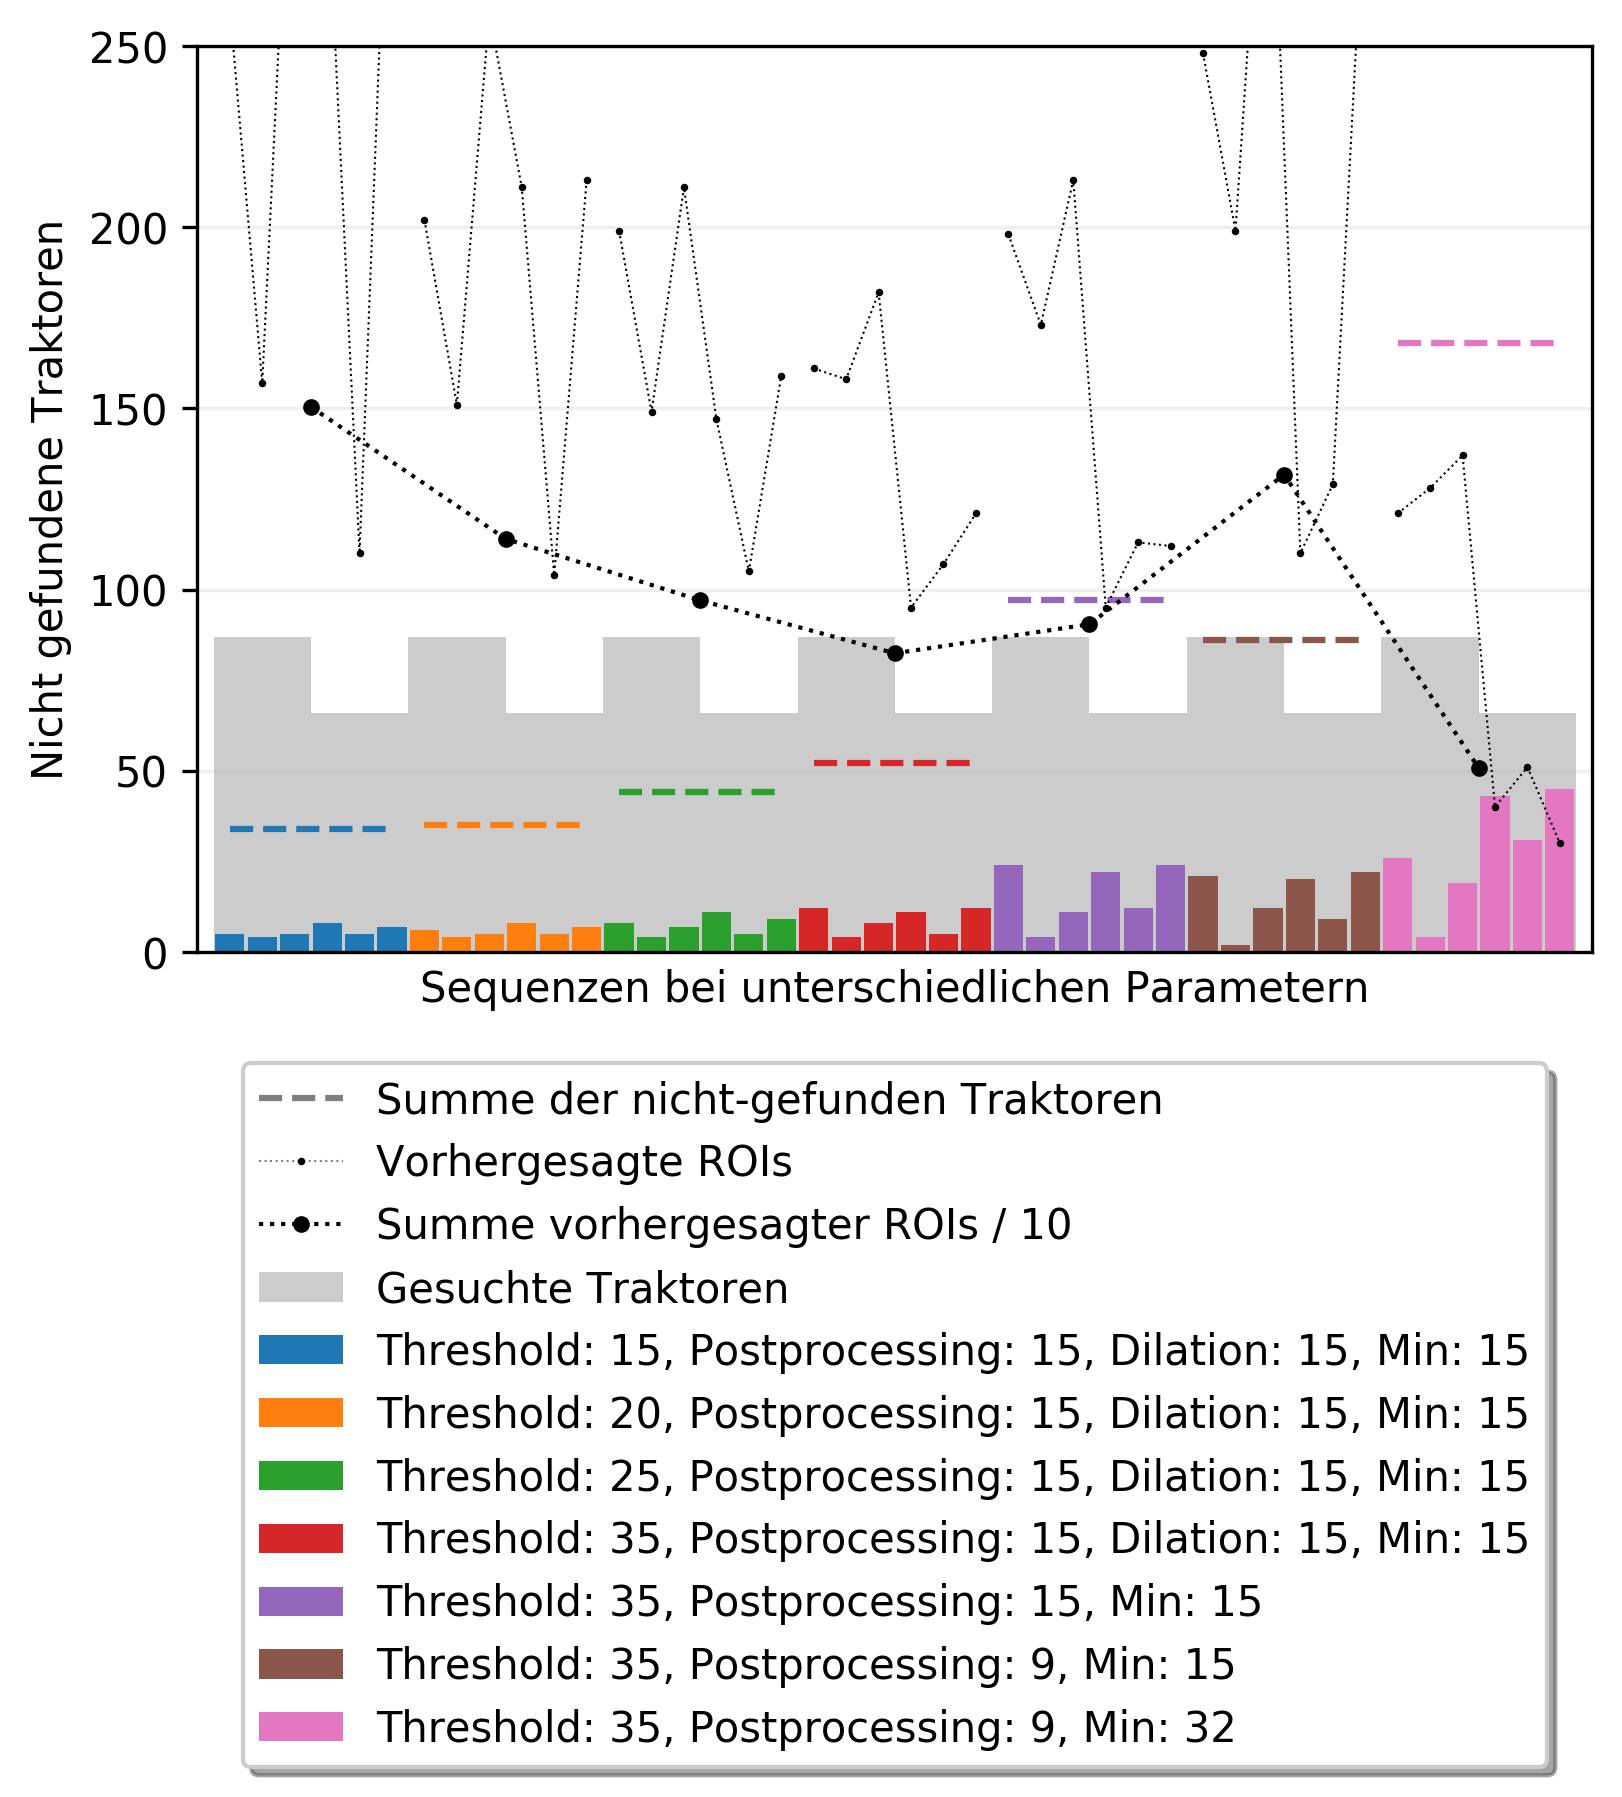
\includegraphics[width=0.95\textwidth]{figures/chapter_6/bgs-opti}
    \caption[Optimierungsschritte für die Background Subtraction]
        {\BF{Optimierungsschritte für die Background Subtraction.}
        Beschreibung des Plots:
        \begin{itemize*}
            \item die Farben entsprechen einer bestimmten Konfiguration
            \item die farbigen Balken entsprechen den jeweils nicht gefundenen Traktoren
            \item die grauen Balken geben die gesuchten Traktoren an
        \end{itemize*}}
    \label{fig:ch6:bgs_opti}
\end{figure}

% *********************************************

\section{Klassifikator} \label{ch6:classifier}
Im Folgenden werden unterschiedliche Varianten des EfficientNets evaluiert.
Die dafür benötigten Metriken werden beschrieben und ein Klassifikationsschwellwert wird bestimmt.

\subsection{Trainingsdaten} \label{ch6:train_data}
Die \acp{ROI} aus insgesamt $3202$ Bildern wurden mit den optimierten Parametern für den \ac{BGS} ausgeschnitten und anschließend händisch klassifiziert.

Die Anzahl der extrahierten \acp{ROI} ist in \autoref{ch6:tab:data} zu sehen.
Dabei fällt auf, dass ein großes Ungleichgewicht zwischen den beiden Klassen besteht.
Es gibt $3.8$ mal mehr \SC{Andere} als \SC{Traktoren}.

\begin{table}[ht]
    \centering
    \begin{tabular}{c|ccc}
    \textbf{Klasse} & \textbf{Insgesamt} & \textbf{Train 75\%} & \textbf{Val 25\%} \\ \shline

    \text{Traktor} & \text{2824} & \text{2125} & \text{708} \\
    \text{Andere}  & \text{10812} & \text{8109} & \text{2703} \\
    \end{tabular}
    \caption{Anzahl der extrahieren ROIs}
    \label{ch6:tab:data}
\end{table}

Beim Trainieren mit unausgeglichenen Datensätzen gibt es mehrere Optionen.
\begin{labeling}{gewichteter Loss\quad}
    \item [\BF{Ignorieren}]
        Nichts weiter machen (wird im Folgenden als \IT{Default} bezeichnet).
    \item [\BF{Gewichteter Loss}]
        Den Loss für die unterrepräsentierte Klasse höher gewichten.
        In diesem Fall mit dem Verhältnis $1$ zu $3.8$.
    \item [\BF{Upsampeln}]
        Die unterrepräsentierte Klasse hochsampeln, indem weitere Augmentationen für sie hinzugefügt werden.
        In diesem Fall werden zwei zusätzliche Bilder für jeden Traktor erstellt: Heller, dunkler und zufällig einer der Operationen Blur, Rauschen oder Farbchannelshift.
        Der hochgesampelte Trainingsdatensatz enthält folglich $8500$ Traktoren.
    \item [\BF{Downsampeln}]
        Die überrepräsentierte Klasse herruntersampeln (Bilder verwerfen).
\end{labeling}

Die ersten drei Optionen werden im Folgenden getestet.
Die letzte Option widerspricht der Prämisse, dass \acp{CNN} aus großen Datenmengen lernen und wird daher nicht verwendet.

Im Durchschnitt sind die extrahierten Traktoren $113x99$ Pixel groß.
Als Basis $\phi$ für das EfficientNet wird deshalb $-5$ gewählt, sodass es eine Inputgröße von $112x112$ Pixel erwartet.
Das Modell wird folgend als \SC{EFN-N5} bezeichnet, sein kleiner Bruder mit $\phi=-6$ als \SC{EFN-N6}, usw.


\subsection{Definitionen für die Evaluation} \label{ch6:defs_cnn}
Es gibt mehrere Metriken zum auswerten eines \ac{ANN}s.
Als Grundlage dient dabei oft die Confusion Matrix.
Aus der Confusion Matrix werden weitere Qualitätsmaße abgeleitet.
Die Matrix und die Qualitätsmaße werden in \autoref{ch6:cm} eingeführt.

Die Grundlagen zum Wählen eines Schwellwerts, der die skalaren Vorhersagen einer (binären) Klasse zuteilt, werden in \autoref{ch6:threshold} aufgezeigt.

\subsubsection{Confusion Matrix} \label{ch6:cm}
Die Confusion Matrix fasst viele relevante Informationen für die Evaluation zusammen.
Die Elemente der Confusion Matrix sind in \autoref{ch5:cm_1} dargestellt.

\begin{table}[ht]
\centering
\begin{tabular}[b]{c|cc}
    \BF{Akronym} & \textbf{Übereinstimmung} & \textbf{Vorhersage} \\ \shline
    TP & \BF{T}rue & \BF{P}ositive \\ \hline
    TN & \BF{T}rue & \BF{N}egative \\ \hline
    FP & \BF{F}alse & \BF{P}ositive \\ \hline
    FN & \BF{F}alse & \BF{N}egative \\
\end{tabular}
\caption{Elemente der Confusion Matrix}
\label{ch5:cm_1}
\end{table}

Zum Beispiel entspricht ein TP demnach einer korrekt klassifizierten landwirtschaftlichen Maschine, während beim FP eine landwirtschaftliche Maschine erkannt wurde, wo keine ist.

Eine beispielhafte Confusion Matrix ist in \autoref{fig:ch6:confusion_matrix} veranschaulicht.
\begin{figure}[ht]
    \center
    \renewcommand\arraystretch{1.5}
    \setlength\tabcolsep{0pt}
    \begin{tabular}{c @{\hspace{0.7em}}>{\bfseries}r @{\hspace{0.7em}}c @{\hspace{0.4em}}c @{\hspace{0.7em}}l}
        \multirow{9}{*}{\rotatebox{90}{\parbox{4.1cm}{\bfseries\centering Richtige Klasse \\}}} & 
            & \multicolumn{2}{c}{\bfseries Vorhersage} & \\
        & & \bfseries P & \bfseries N & \bfseries \\
        & P & \MyBox{$TP=1$} & \MyBox{$FN=8$} \\[2.4em]
        & N & \MyBox{$FP=1$} & \MyBox{$TN=90$}
    \end{tabular}
    \caption{Confusion Matrix - Beispiel}
    \label{fig:ch6:confusion_matrix}
\end{figure}

Aus diesen vier Kriterien lassen sich Qualitätsmaße ableiten.

Wie in Tabelle \autoref{ch6:tab:metrics} zu sehen, vermittelt die Genauigkeit (engl. Accuracy) fälschlicherweise den Eindruck, dass die Vorhersagen aus \autoref{fig:ch6:confusion_matrix} gut sind.
Aber in Wirklichkeit werden positive Klassen nur zu \SI{11}{\percent} richtig erkannt (\ac{TPR} oder Recall genannt).
Daher ist bei unausgeglichenen Datensätzen die \IT{Accuarcy} als alleinige Metrik nicht geeignet.
% Daher sollte bei unausgeglichenen Datensätzen auch die \IT{Balanced Accuracy} bestimmt werden, welche sowohl die \ac{TPR} als auch die \ac{TNR} berücksichtigt.

\begin{table}[ht]
    \centering
    \def\arraystretch{1.3}
    % \def\arraystretch{2}\tabcolsep=10pt
    % \setlength{\extrarowheight}{5em}
    \begin{tabular}[c]{l|c|c}
        \BF{Qualitätsmaß} & \textbf{Formel} & \BF{Beispiel} \\ \shline
        Accuracy & $\frac{TP + TN}{TP+FP+TN+FN}$ & $\frac{1+90}{1+1+90+8}=0.91$ \\ \hline
        \ac{TNR} / Specifity & $\frac{TN}{TN+FP}$ & $\frac{90}{90+1}=0.99$ \\ \hline
        \ac{FPR} & $\frac{FP}{FP+TN} = 1 - TNR$ & $1 - 0.99 = 0.01$ \\ \hline
        \ac{TPR} / Recall & $\frac{TP}{TP+FN}$ & $\frac{1}{1+8}=0.11$ \\ \hline
        % Balanced Accuracy & $\frac{TPR + TNR}{2}$ & $\frac{0.11 + 0.99}{2}=0.55$ \\ \hline
        Precision & $\frac{TP}{TP+FP}$ & $\frac{1}{1+1}=0.5$ \\ \hline
        F1 Score & $2 \cdot \frac{precision \cdot recall}{precision + recall}$ & $2 \cdot \frac{0.5 \cdot 0.11}{0.5 + 0.11}=0.18$
    \end{tabular}.
    \caption[Berechnung der Qualitätsmaße]{Berechnung der Qualitätsmaße - bei einem idealen Klassifikator gehen alle Metriken (bis auf die \ac{FPR}) gegen $1$.}
    \label{ch6:tab:metrics}
\end{table}

Ein weiteres Maß ist die Precision.
Diese gibt an, wie viel Prozent der positiv Identifizierten wirklich positiv sind.

Vorteil von Precision und Recall ist, dass diese nicht die TNs mit einbeziehen und sich deshalb für die Bewertung eines unbalancierten Datensatzes eignen.
Allerdings steht die Precision mit dem Recall in Konflikt: Verbessern der Precision senkt den Recall und vice versa.
Denn erhöht man den Schwellwert, der bestimmt ab wann die Vorhersage als positiv gewertet wird, sinken zwar die FPs, aber die FNs steigen und der Recall verschlechtert sich.
Um Recall und Precision in ein Gleichgewicht zu bringen, wird der F1 Score berechnet, welcher die harmonische Mitte beider Werte bestimmt.

\subsubsection{Schwellwert bestimmen: ROC und Precision-Recall Kurve} \label{ch6:threshold}
Die ROC-Kurve zeigt die Performanz eines Modells für alle Klassifikationsschwellwerte.
Die Kurve stellt die zwei Parameter \ac{TPR} (y-Achse) und \ac{FPR} (x-Achse) bei unterschiedlichen Schwellwerten gegenüber.

Wird der Schwellwert gesenkt, werden mehr Vorhersagen als positiv klassifiziert, sodass die FPs und TPs steigen.
Die \autoref{ch6:fig:curves} zeigt links eine typische ROC Kurve.

\begin{figure}[ht]
    \centering
    \subfloat[\SC{a.} ROC Kurve]{{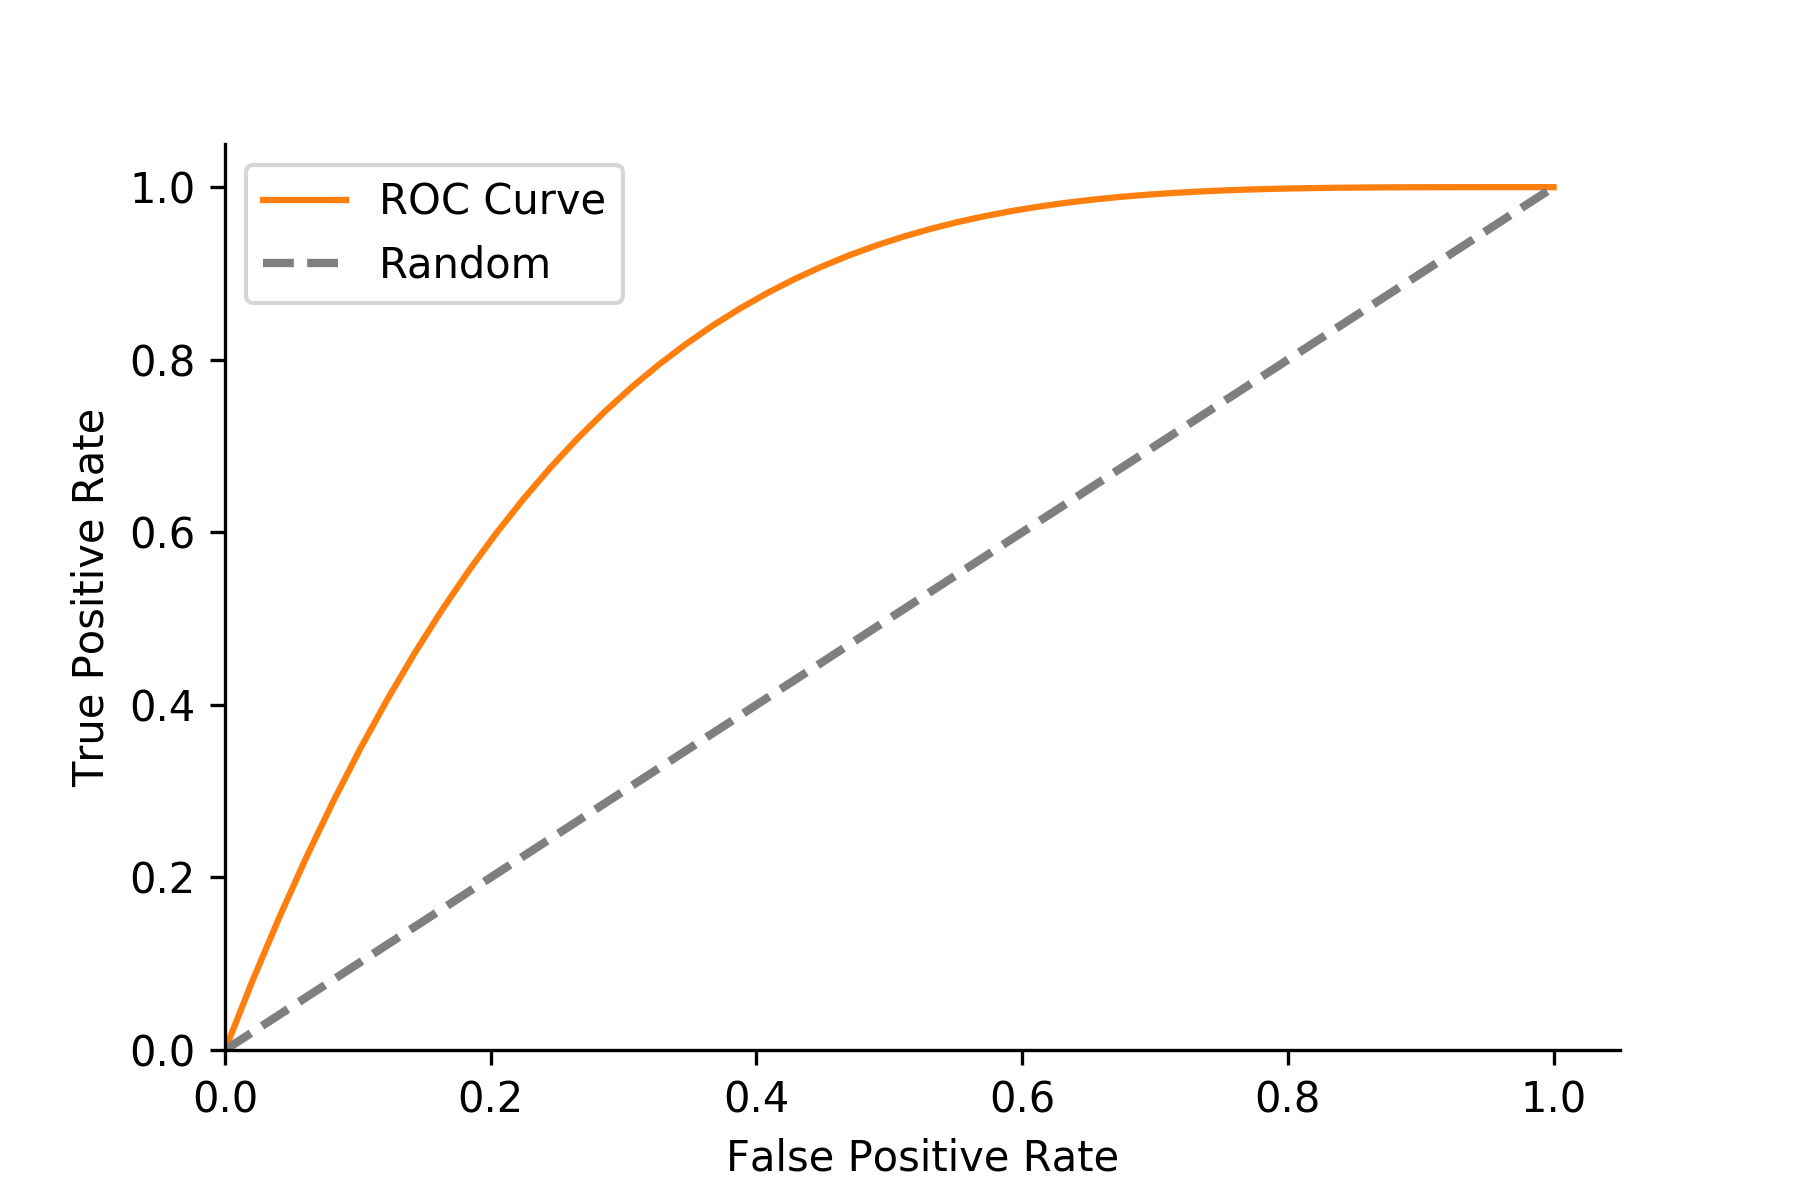
\includegraphics[width=.5\textwidth]{figures/chapter_6/roc_curve}}}
    \subfloat[\SC{b.} Precision-Recall Kurve]{{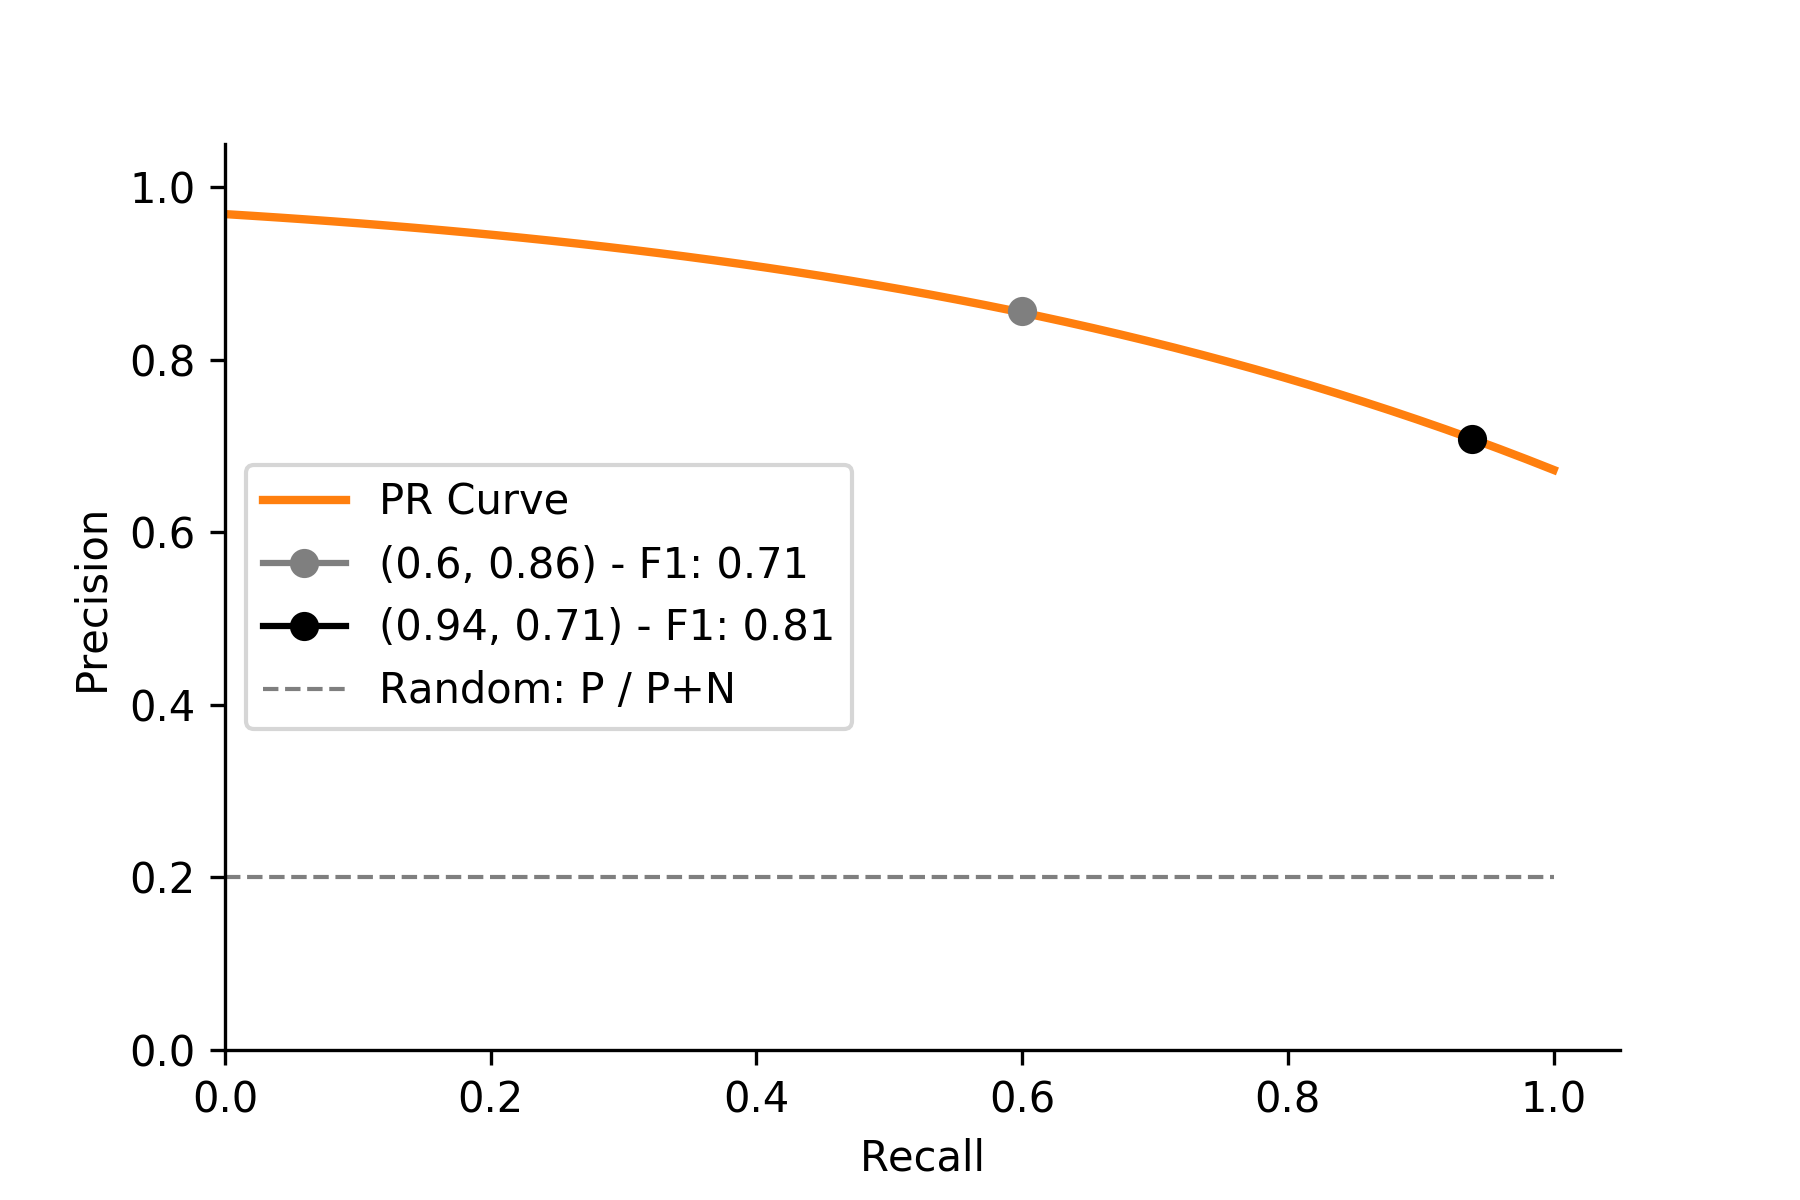
\includegraphics[width=.5\textwidth]{figures/chapter_6/pr_curve}}}
    \caption[Beispielhafte ROC / PR Kurven]{Beispielhafte Performanzkurven.
    \SC{a.} zeigt eine gute ROC Kurve, da sie eindeutig über der Basislinie liegt.
    \SC{b.} zeigt eine gute PR Kurve, welche ebenfalls eindeutig über der Basis $y=0.2$ liegt. }
    \label{ch6:fig:curves}
\end{figure}

Bei einem ausgeglichenen Datensatz trifft ein Zufallsklassifikator durchschnittlich zu 50 Prozent die richtige Vorhersage.
Deshalb wird als Referenz eine diagonale Basislinie genommen.
Ein perfektes Modell dagegen hat eine \ac{TPR} von $1$ und eine \ac{FPR} von $0$.
Das ist allerdings unrealistisch, weshalb der Schwellwert auf der Kurve gewählt werden kann, der die kleinste Distanz zu $(0,1)$ aufweist.

\bigskip
Jedoch gilt für die ROC Kurve, dass diese nur für ausbalancierte Datensätze geeignet ist.
Um die Performanz für unbalancierte Datensätze visuell zu evaluieren und einen Schwellwert zu wählen, wird daher eine Precision-Recall Kurve erstellt \cite{saito_precision-recall_2015}.

\autoref{ch6:fig:curves} zeigt eine Precision-Recall Kurve.
Der Punkt $(0.6, 0.86)$ zeigt die Performanz des Modells bei einem bestimmtem Schwellwert: Es hat einen Recall von $0.6$ und eine Precision von $0.86$.
Also findet es $60$\% aller Positiven, wobei $86$\% der positiven Vorhersagen korrekt sind.
Je nach Anwendungsfall kann es sein, dass entweder der Recall oder die Precision hoch sein soll.
So hat der Punkt $(0.94, 0.71)$ auf dieser Kurve den höchsten F1 Wert.
Bei seinem niedrigeren Schwellwert werden $94$\% aller Positiven gefunden, jedoch werden dabei auch $29$\% fälschlicherweise als positiv klassifiziert.

Die \IT{Average Precision} fasst die Precision-Recall Kurve zusammen, sodass Modelle direkt miteinander verglichen werden können.
Dazu werden die Precisions für jeden der $N$ Thresholds aufsummiert und mit dem Anstieg des Recalls gewichtet:
\begin{flalign}
    AP = \sum_{n=1}^N{(R_n - R_{n-1}) \cdot P_n}
\end{flalign}

\subsection{Ergebnisse}
Zum Trainieren des \SC{EFN-N5} wurden zuerst, wie in \autoref{ch5:cnn:train} beschrieben, die minimalen und maximalen Lernraten bestimmt.
Dies geschah für $9$ Grundaufstellungen: 
\begin{itemize}
    \item Default, gewichteter Loss und hochgesampelter Trainingsdatensatz
    \item mit jeweils einem Dropout von $0.1, 0.125$ oder $0.15$.
\end{itemize}

Beim Bestimmen der Lernraten hat sich gezeigt, dass die maximale Lernrate für die unterschiedlichen Dropoutraten fast gleich ist.
Für die drei Arten zum Umgang mit dem unausgeglichenen Datensatz unterscheiden sich die maximalen Lernraten allerdings:

\begin{itemize*}
    \item Default: $0.1669$,
    \item gewichteter Loss: $0.2002$ und
    \item hochgesampelt: $0.2673$.
\end{itemize*}

Alle Konfiguration fangen direkt an zu lernen, sodass eine minimale Lernrate von $0.001$ gewählt wird.
Die Plots zum Lernratentest sind in \autoref{apx:lr_rangetest} zu sehen.

In \autoref{fig:ch6:efn_pr-curve} sind die Precision-Recall Kurven gezeigt.
Alle Konfiguration erzielen sehr gute und fast identische Ergebnisse.

Es wird die höchste der getesteten Dropoutraten gewählt, da diese Modelle am besten generalisieren.

\begin{figure}[ht]
    \begin{small}
        \begin{center}
            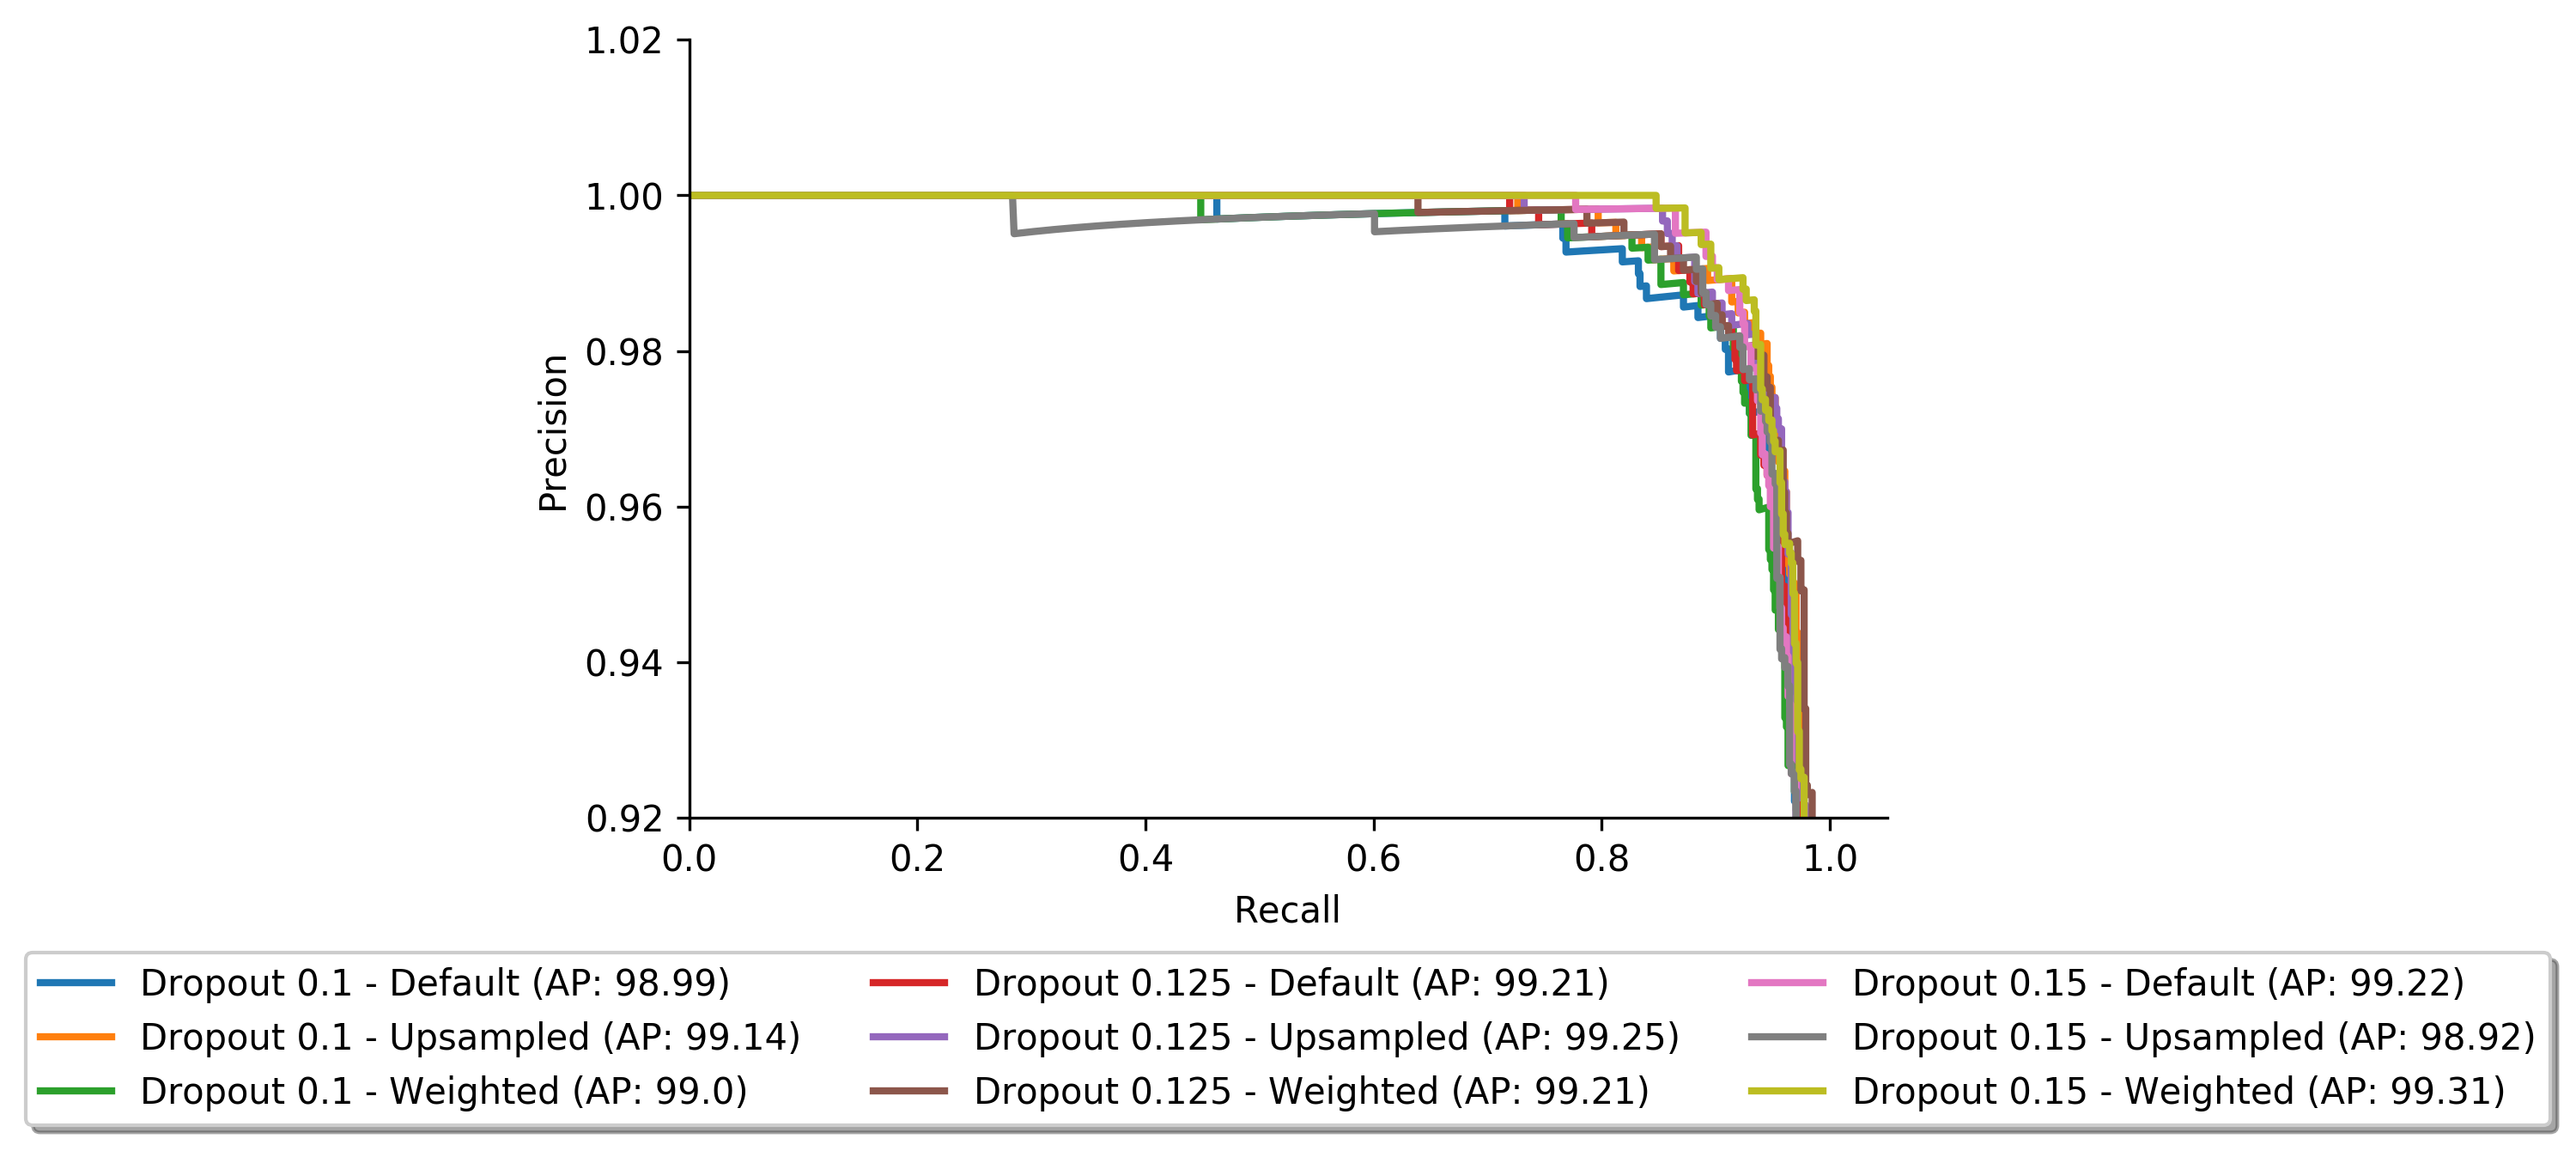
\includegraphics[width=0.95\textwidth]{figures/chapter_6/efnN5-pr_curve}
        \end{center}
        \caption{Precision-Recall Kurven für alle getesteten Konfigurationen}
        \label{fig:ch6:efn_pr-curve}
    \end{small}
\end{figure}

In \autoref{fig:ch6:efn_pr-curve2} sind die Ergebnisse nochmals für die Modelle mit einer Drop\-out\-rate von $0.15$ aufgezeigt.
Aufgrund des stark erhöhten Lernaufwands für die hochgesampelte Methode und der sogar leicht reduzierten AP, scheidet diese Konfiguration ebenfalls aus.
Die besten Ergebnisse erzielte die Konfiguration mit dem gewichteten Loss.
Bei einem Klassifikationsschwellwert von $0.573$ hat dieses Modell den höchsten F1 Wert, welcher deshalb für die weitere Evaluation verwendet wird.

\begin{figure}[H]
    \begin{small}
        \begin{center}
            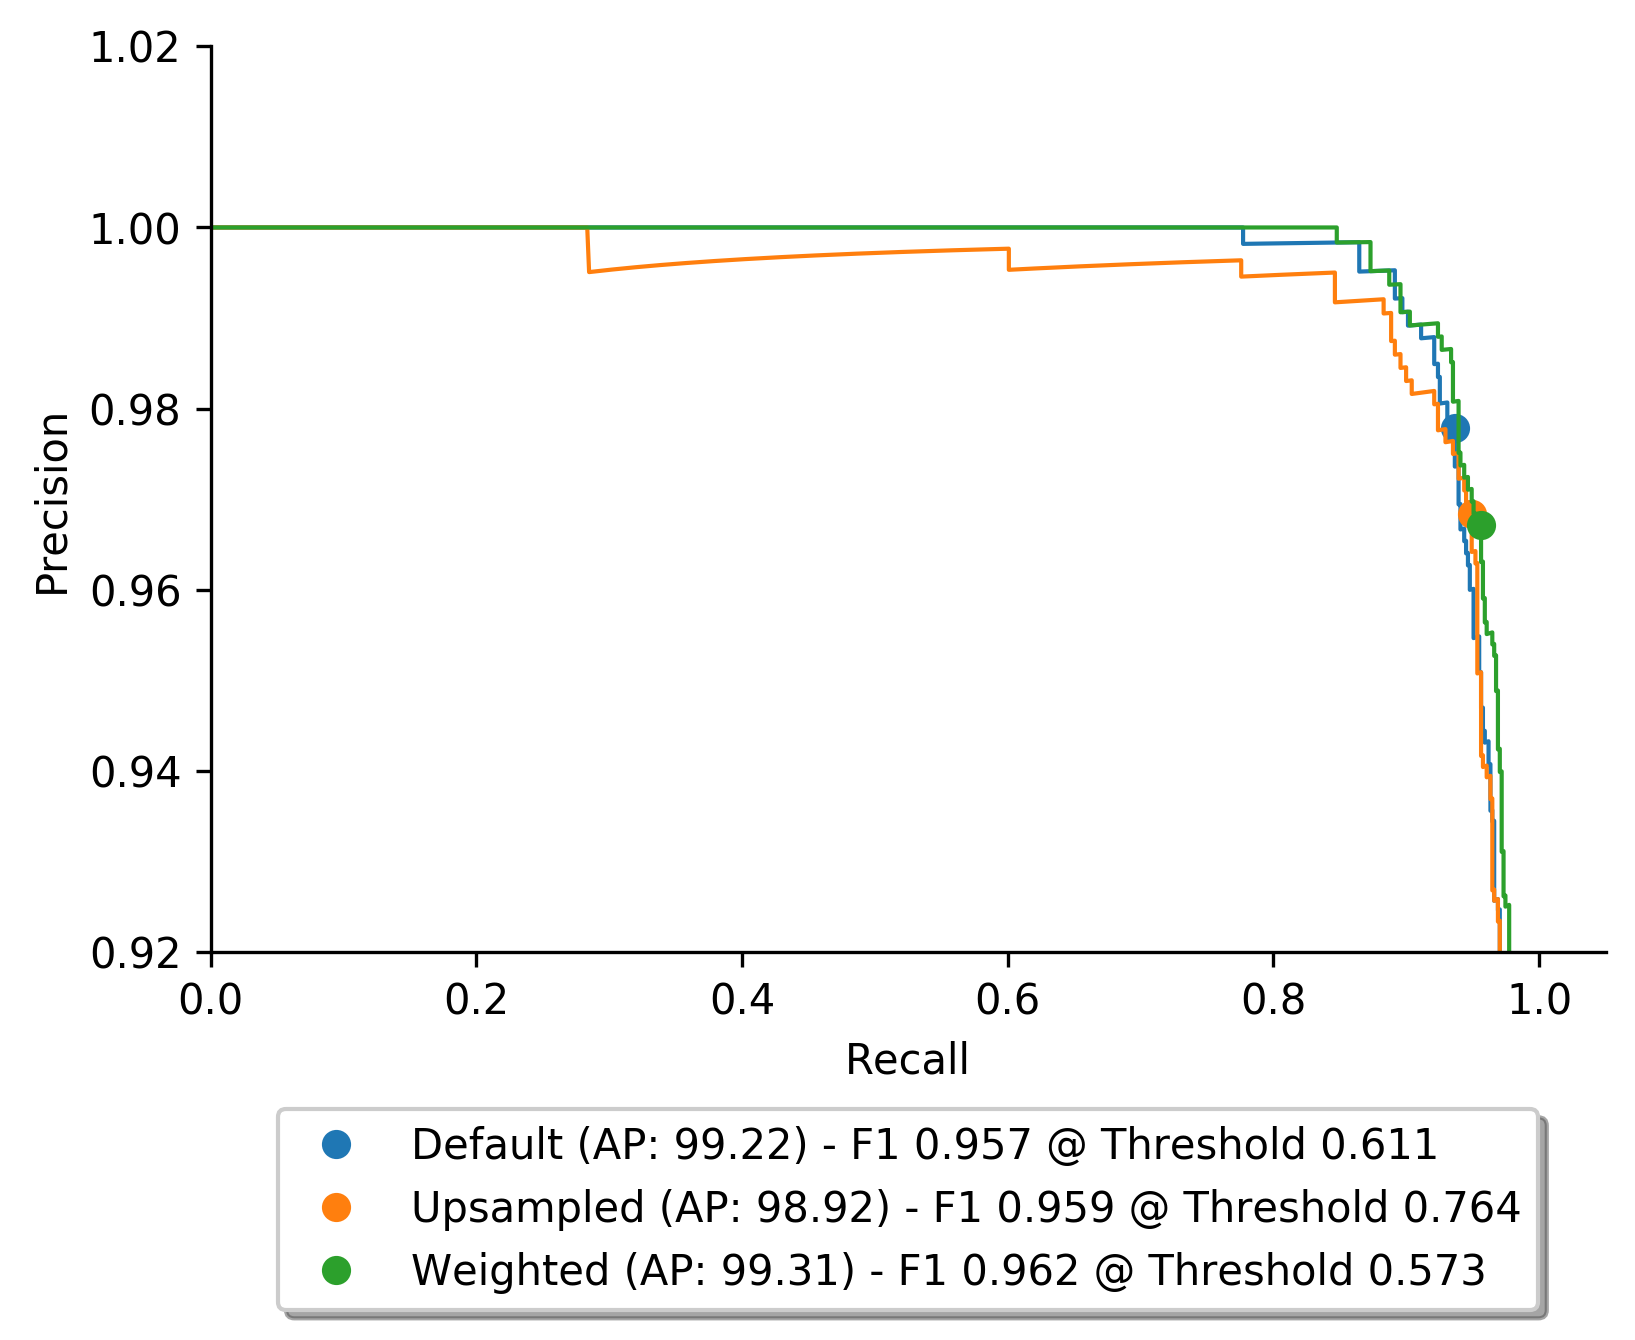
\includegraphics[width=0.95\textwidth]{figures/chapter_6/efnN5-pr_curve2}
        \end{center}
        \caption{Precision-Recall Kurven für Dropout von $0.15$}
        \label{fig:ch6:efn_pr-curve2}
    \end{small}
\end{figure}


% - Unbalanced Methoden
% - Threshold

% - Runterskaliert bis X

% \begin{table}[ht]
%     \centering
%     \begin{tabular}{c||cccc|cc}
%     \textbf{Model} &

%     \textbf{Accuarcy} &
%     \textbf{Recall} &
%     \textbf{Precision} &
%     \textbf{F1} &

%     \textbf{Latency} &
%     \textbf{Latency TensorRT} \\ \shline

%     EFN-N4 & \bf 0 & \bf 0 & \bf 0 & \bf 0 & 0 & 0 \\
%     EFN-N9 & 0 & 0 & 0 & 0 & \bf 0 & \bf 0 \\

%     \end{tabular}
%     \caption{Ergebnisse CNN}
%     \label{ch5:tab:erg1}
% \end{table}

% ********************************************* RESULTS
\section{Inferenztest} \label{ch6:inference}
Bisher wurden die Komponenten einzeln evaluiert.
Ob das Konzept sich letztlich eignet und eine effektive Lösung darstellt, hängt allerdings vom Zusammenspiel von \ac{BGS} und \ac{CNN} ab.
Zur finalen Evaluation werden daher beide Komponenten in Kette geschaltet und getestet.
Das ist vergleichbar mit einem Test zur Inferenzlaufzeit, da beide Komponenten auf ungesehenen Daten arbeiten.

\bigskip
Es werden drei fünfminütige Aufnahmen erstellt und annotiert:
\begin{labeling}{Nacht \quad}
    \item [\BF{Tag}]
        Aufnahmen bei Tag mit unterschiedlichen Traktoren.
        Insgesamt gibt es 109 sich bewegende Traktoren.
    \item [\BF{Nacht}]
        Aufnahmen bei Nacht und aktiven Scheinwerfern.
        Insgesamt werden 133 Traktoren gesucht.
    \item [\BF{Tiere}] 
        Aufnahmen bei Tag, wobei sich überwiegend Tiere auf dem Feld bewegen.
        Insgesamt werden deshalb nur 33 Traktoren gesucht.
\end{labeling}
Für alle drei Aufnahmen werden die Wettereinwirkungen Nebel und Regen simuliert.

\bigskip
Für die Auswertung gilt Folgendes:
\begin{labeling}{False Positive (FP)\quad}
    \item [\BF{Nicht gefunden}]
        Vom \ac{BGS} wird der Traktor nicht gefunden oder wird bei der Blobanalyse herausgefiltert.
    \item [\BF{\ac{TP}}]
        Ein Traktor wird gefunden und vom \ac{CNN} als solcher klassifiziert.
    \item [\BF{\ac{FP}}]
        Vom \ac{CNN} wird ein Traktor für eine \ac{ROI} vorhergesagt, obwohl sich dort kein Traktor befindet.
    \item [\BF{\ac{FN}}]
        Das \ac{CNN} hat für eine \ac{ROI} keinen Traktor vorhergesagter, obwohl es sich um einen handelt.
        Für die finale Analyse werden die \acp{FN} mit den nicht gefundenen Traktoren addiert, da in beiden Fällen fälscherlicherweise kein Traktor hervorgesagt wird.
    \item [\BF{\ac{TN}}]
        Alle Bewegungen die vom \ac{BGS} erkannt werden, jedoch keine Traktoren sind und auch nicht als solche klassifiziert werden.
\end{labeling}

\bigskip
In \autoref{ch6:tab:inf_cm} sind die Ergebnisse numerisch und in \autoref{ch6:fig:inf_cm} visuell dargestellt.

\begin{table}[ht]
    \centering
    \begin{tabular}{cl||ccc|cccc}
    \textbf{} &
    \textbf{Sequenz} &
    \BF{\acp{ROI}} &
    \BF{gesucht} &
    \BF{nicht gefunden} &
    \BF{\acp{TP}} &
    \BF{\acp{FP}} &
    \BF{\acp{FN}} &
    \BF{\acp{TN}} \\ \shline

    \parbox[t]{2mm}{\multirow{3}{*}{\rotatebox[origin=c]{90}{Tag}}} &
      Nebel      & 183 & 109 & 5     & 101 & 5 & 3  & 69 \\
    & Original   & 202 & 109 & 4     & 103 & 4 & 2  & 89 \\
    & Regen      & 220 & 109 & 6     & 102 & 6 & 2  & 104 \\ \hline

    \parbox[t]{2mm}{\multirow{3}{*}{\rotatebox[origin=c]{90}{Nacht}}} &
      Nebel      & 442 & 133 & 5      & 127 & 5  & 1  & 304 \\
    & Original   & 235 & 133 & 10     & 122 & 10 & 1  & 92  \\
    & Regen      & 302 & 133 & 7      & 125 & 7  & 1  & 162 \\ \hline

    \parbox[t]{2mm}{\multirow{3}{*}{\rotatebox[origin=c]{90}{Tiere}}} &
      Nebel      & 85  & 33 & 3     & 30 & 3 & 0 & 49 \\
    & Original   & 90  & 33 & 1     & 32 & 1 & 0 & 56 \\
    & Regen      & 162 & 33 & 1     & 32 & 1 & 0 & 128 \\ \hline
    \end{tabular}
    \caption{Ergebnisse BGS und CNN}
    \label{ch6:tab:inf_cm}
\end{table}

\begin{figure}[ht]
    \begin{small}
        \begin{center}
            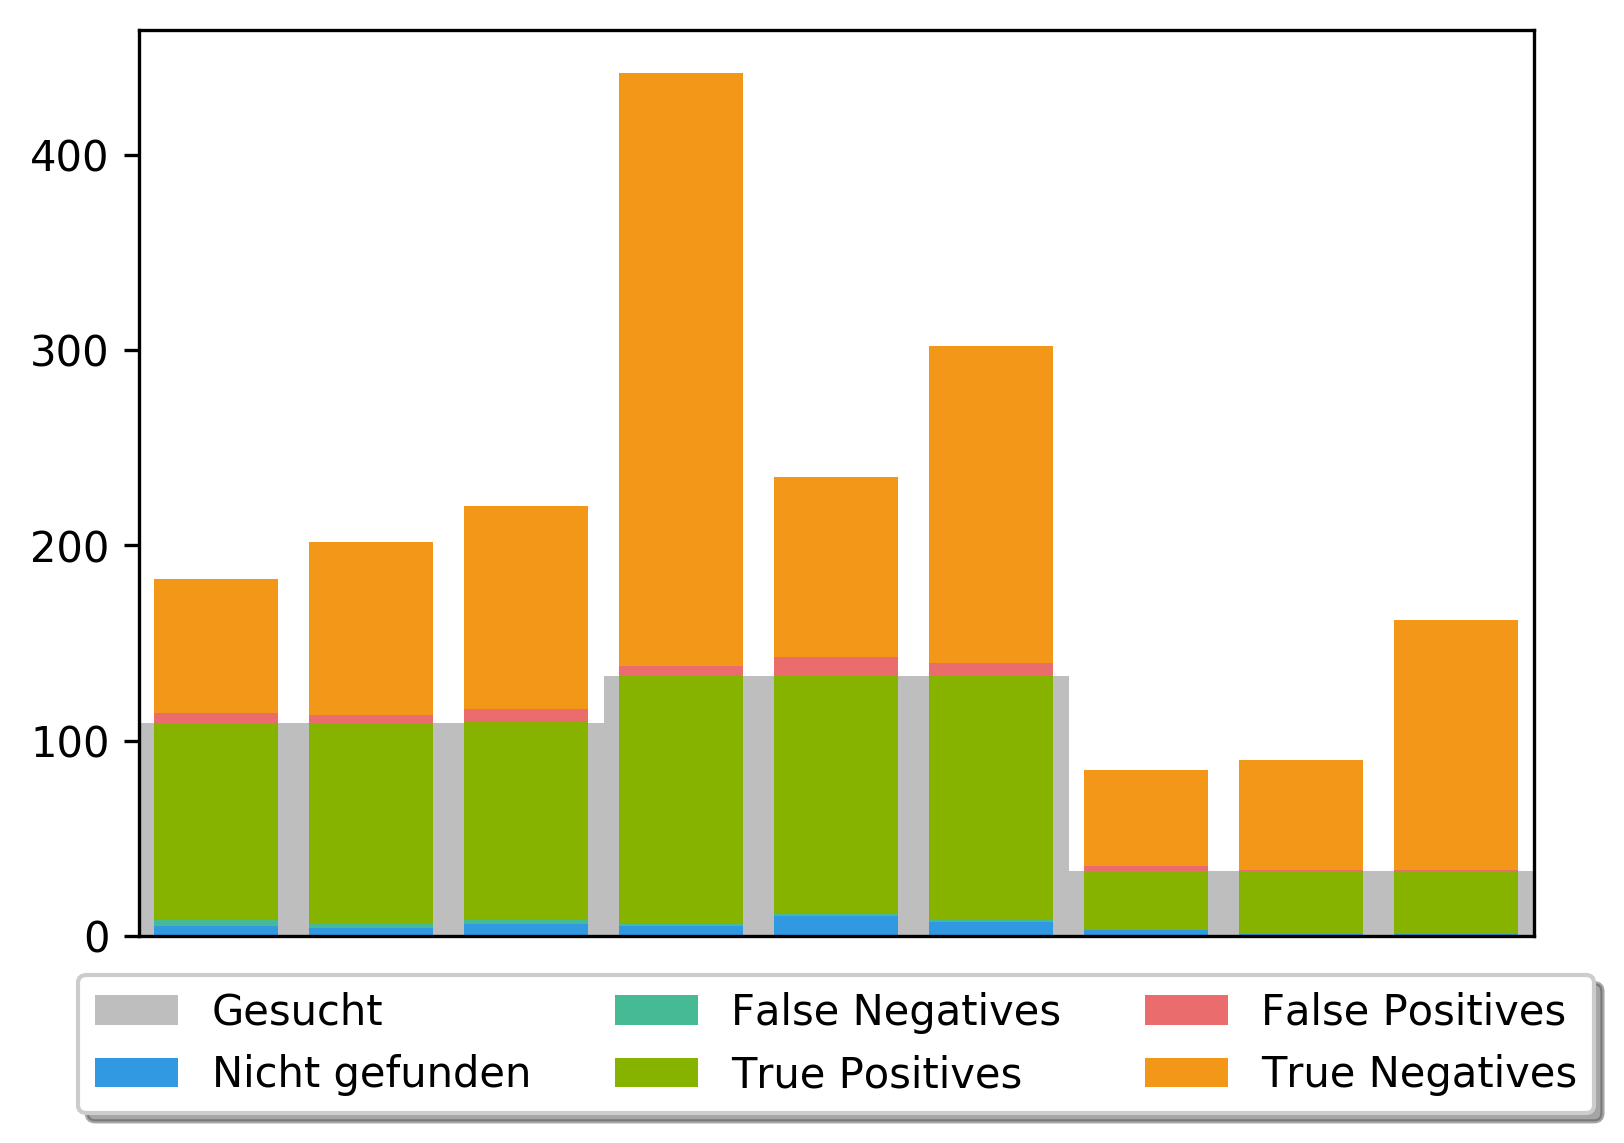
\includegraphics[width=0.95\textwidth]{figures/chapter_6/inference-cmbars}
        \end{center}
        \caption[Inferenztest - Confusion Matrix in Balkenformat]
        {Inferenztest - Confusion Matrix in Balkenformat (Reihenfolge entspricht der selben wie in \autoref{ch6:tab:inf_cm})}
        \label{ch6:fig:inf_cm}
    \end{small}
\end{figure}

Für die Ergebnismetriken aus \autoref{ch6:fig:inf_metrics} wurden die nicht gefundenen Traktoren und die \acp{FN} summiert.
Beide Komponenten erzielen dabei sehr gute Ergebnisse.
Es werden insgesamt $94.9 \%$ der Trakoren gefunden und richtig klassifiziert.
Gleichzeitig sind nur $6.3 \%$ der als Traktor identifizierten \acp{ROI} in Wirklichkeit keine Traktoren.
Das bedeutet, wenn für zwei aufeinanderfolgende Bilder ein Traktor klassifiziert wurde, die Wahrscheinlichkeit, dass sich kein Traktor auf der Wiese befindet, mit $0.063^2=0.004$ unter einem Prozent liegt.

\begin{figure}[H]
    \begin{small}
        \begin{center}
            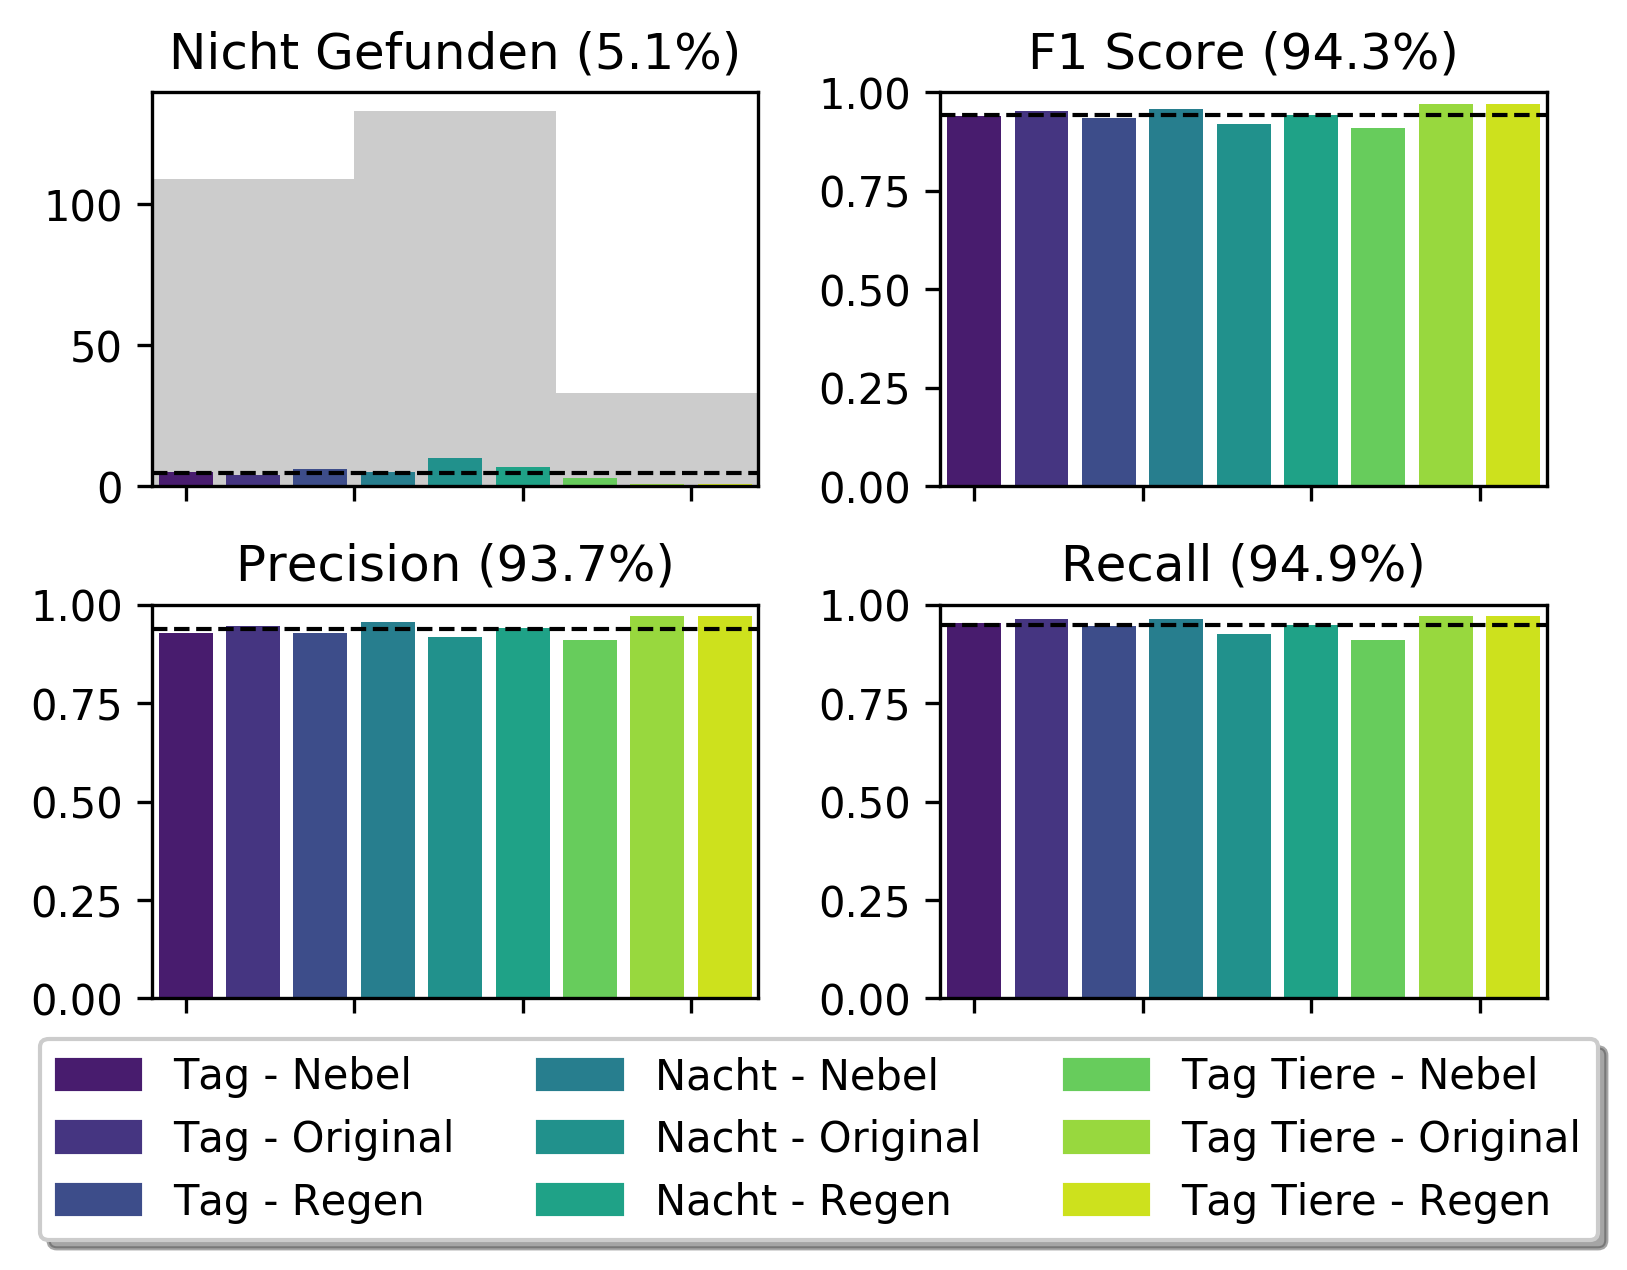
\includegraphics[width=0.95\textwidth]{figures/chapter_6/inference-metrics}
        \end{center}
        \caption[Inferenztest - Ergebnismetriken]
        {Inferenztest - Ergebnismetriken}
        \label{ch6:fig:inf_metrics}
    \end{small}
\end{figure}


\section{Objektgröße und Geschwindigkeit} \label{ch6:scale}
Zuletzt wird untersucht, welche Größe die Traktoren im Bild einnehmen müssen, um
\begin{enumerate*}[(\arabic*)]
    \item vom \ac{BGS} gefunden und
    \item vom \ac{CNN} erkannt zu werden.
\end{enumerate*}

Ein kleine Objektgröße hat mehrere unterschiedliche Implikationen:
\begin{itemize}
    \item Bei der Kamerawahl ist eine geringere Auflösung oder ein höherer Öffnungswinkel möglich.
    \item Bei kleinerem Bild ist der \ac{BGS} schneller, da im Falle von \ac{BMOG} für weniger Pixel ein Mixture Modell erstellt und gepflegt werden muss.
    \item Das \ac{CNN} ist schneller, da im Falle von EfficientNet $\phi$ reduziert werden kann und somit die Anzahl der Berechnungen sinkt.
\end{itemize}


\subsection*{Finden}
Zum Beantworten der ersten Frage wurden die Bilder herunterskaliert, bevor der \ac{BGS} nach Bewegungen sucht.
Die Skalierung geschah von $100$\% bis $10$\% der Originalgröße in Zehnerschritten.
Dementsprechend wurde das Bild in Breite und Höhe um jeweils $10$\% verkleinert.
Dabei wurden ebenfalls die Parameter Postprocessing, Dilatationenanzahl und Mindestgröße für Blobanalyse sukzessive reduziert.
Die genauen Parameter sind in \autoref{apx:bmog_scale} gelistet.

In \autoref{ch6:fig:bgs_scale} sind die jeweiligen Ergebnisse der Skalierung zu sehen.
Bei der Mindest-\ac{IoU} für die Übereinstimmung hat sich erneut gezeigt, dass die gefundenen \acp{ROI} kleinere \acp{IoU} aufweisen.
Das hat sich vor allem bei den kleineren Skalierungen niedergeschlagen, weshalb die Mindestübereinstimmung erneut gesenkt wurde.
Bei einer \ac{IoU} von $0.3$ respektive $0.2$ werden bis zu einer Bildskalierung von $50$\% knapp $95$\% aller Traktoren gefunden.
Für jede weitere Skalierung verdoppelen sich die Fehlvorhersagen stetig.

Hierbei ist zu erwähnen, dass eine Skalierung von $50$\% nicht zu einer Halbierung, sondern zu einer Viertelung der Pixelanzahl führt, da das Bild sowohl in Breite als auch Höhe halbiert wird.
Ein Bild der Auflösung $3264 \times 2448$ ist nach Skalierung also nur noch $1632 \times 1224$ Pixel groß.

Durch die Viertelung nehmen weit entfernte und noch gefundene Traktoren (ohne Anhänger) stichprobenhaft zwischen $28 \times 28$ und $34 \times 34$ Pixel im Bild ein.

\begin{figure}[ht]
    \begin{small}
        \begin{center}
            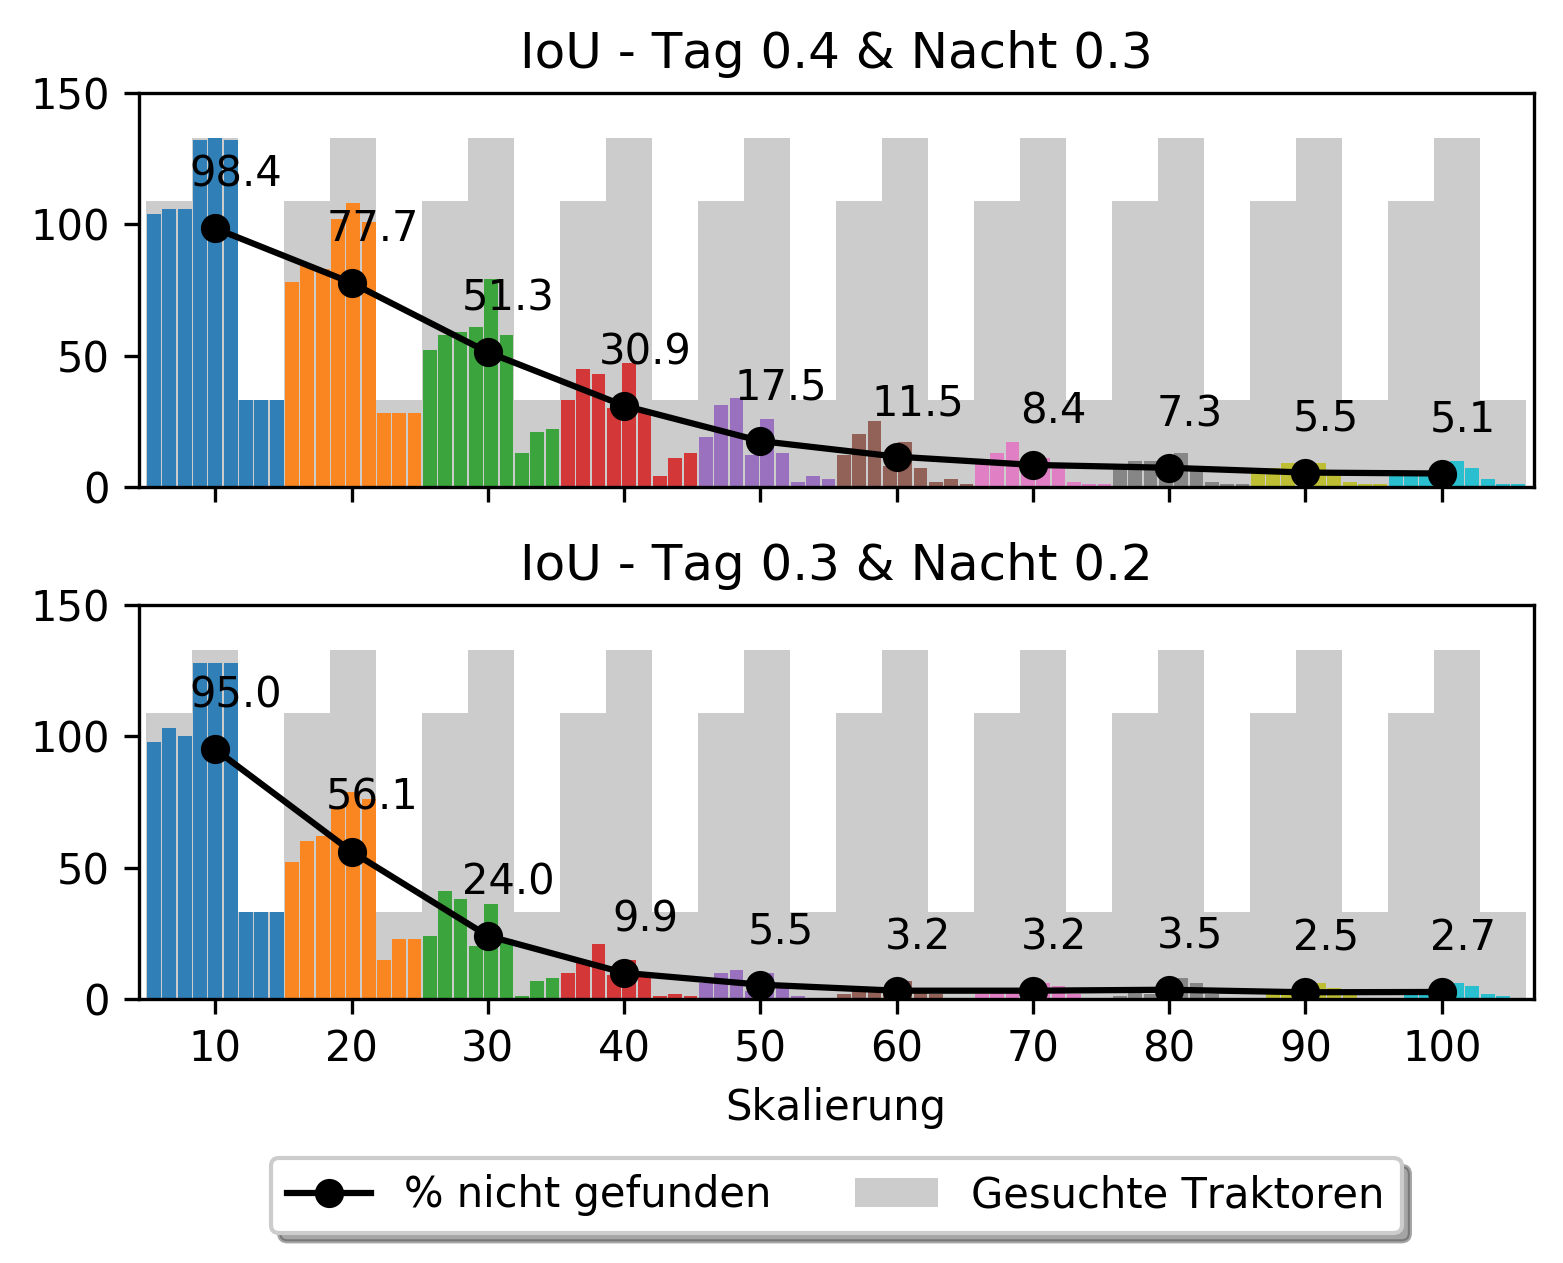
\includegraphics[width=0.95\textwidth]{figures/chapter_6/bgs-scaling}
        \end{center}
        \caption[BGS - Eingangsbildskalierung]
            {BGS - Eingangsbildskalierung bei \IT{hoher} und \IT{niedriger} \ac{IoU}. \\
            Beschreibung des Plots:
            \begin{itemize*}
                \item Farben kennzeichnen Ergebnisse einer Skalierung
                \item Jeder farbige Balken zeigt nicht gefundene Traktoren 
                \item Reihenfolge der Balken entspricht der Reihenfolge aus \autoref{ch6:fig:inf_metrics}
            \end{itemize*}
        }
        \label{ch6:fig:bgs_scale}
    \end{small}
\end{figure}

\subsection*{Erkennen}
Zum Beantworten der zweiten Frage werden weitere EfficientNets mit schrumpfenden Koeffizienten $\phi$ erstellt.
Das geschieht bis zu ~$\phi=-15$, da die Auflösung der Eingangsbilder dann nur noch $26 \times 26$ Pixel beträgt.
Eine weitere Skalierung ist zum Beantworten der übergeordneten Frage \IT{"Wie groß müssen die Objekte sein?"} nicht notwendig.

\bigskip
In Anlehnung des originalen EfficientNets werden die Dropoutraten linear bis $0.05$ reduziert.
Für das Training wurde zuerst für die verschiedenen $\phi$ ein Lernraten Rangetest druchgeführt.
Ergebnis dessen ist eine maximale Lernrate von $0.2002$ (vgl. \autoref{fig:apx:lr_down}).

In \autoref{ch6:fig:efn_scale} sind die Precision-Recall Kurven und der jeweils höchste F1 Wert der kleineren \SC{EFN}s zu sehen.

\begin{figure}[ht]
    \begin{small}
        \begin{center}
            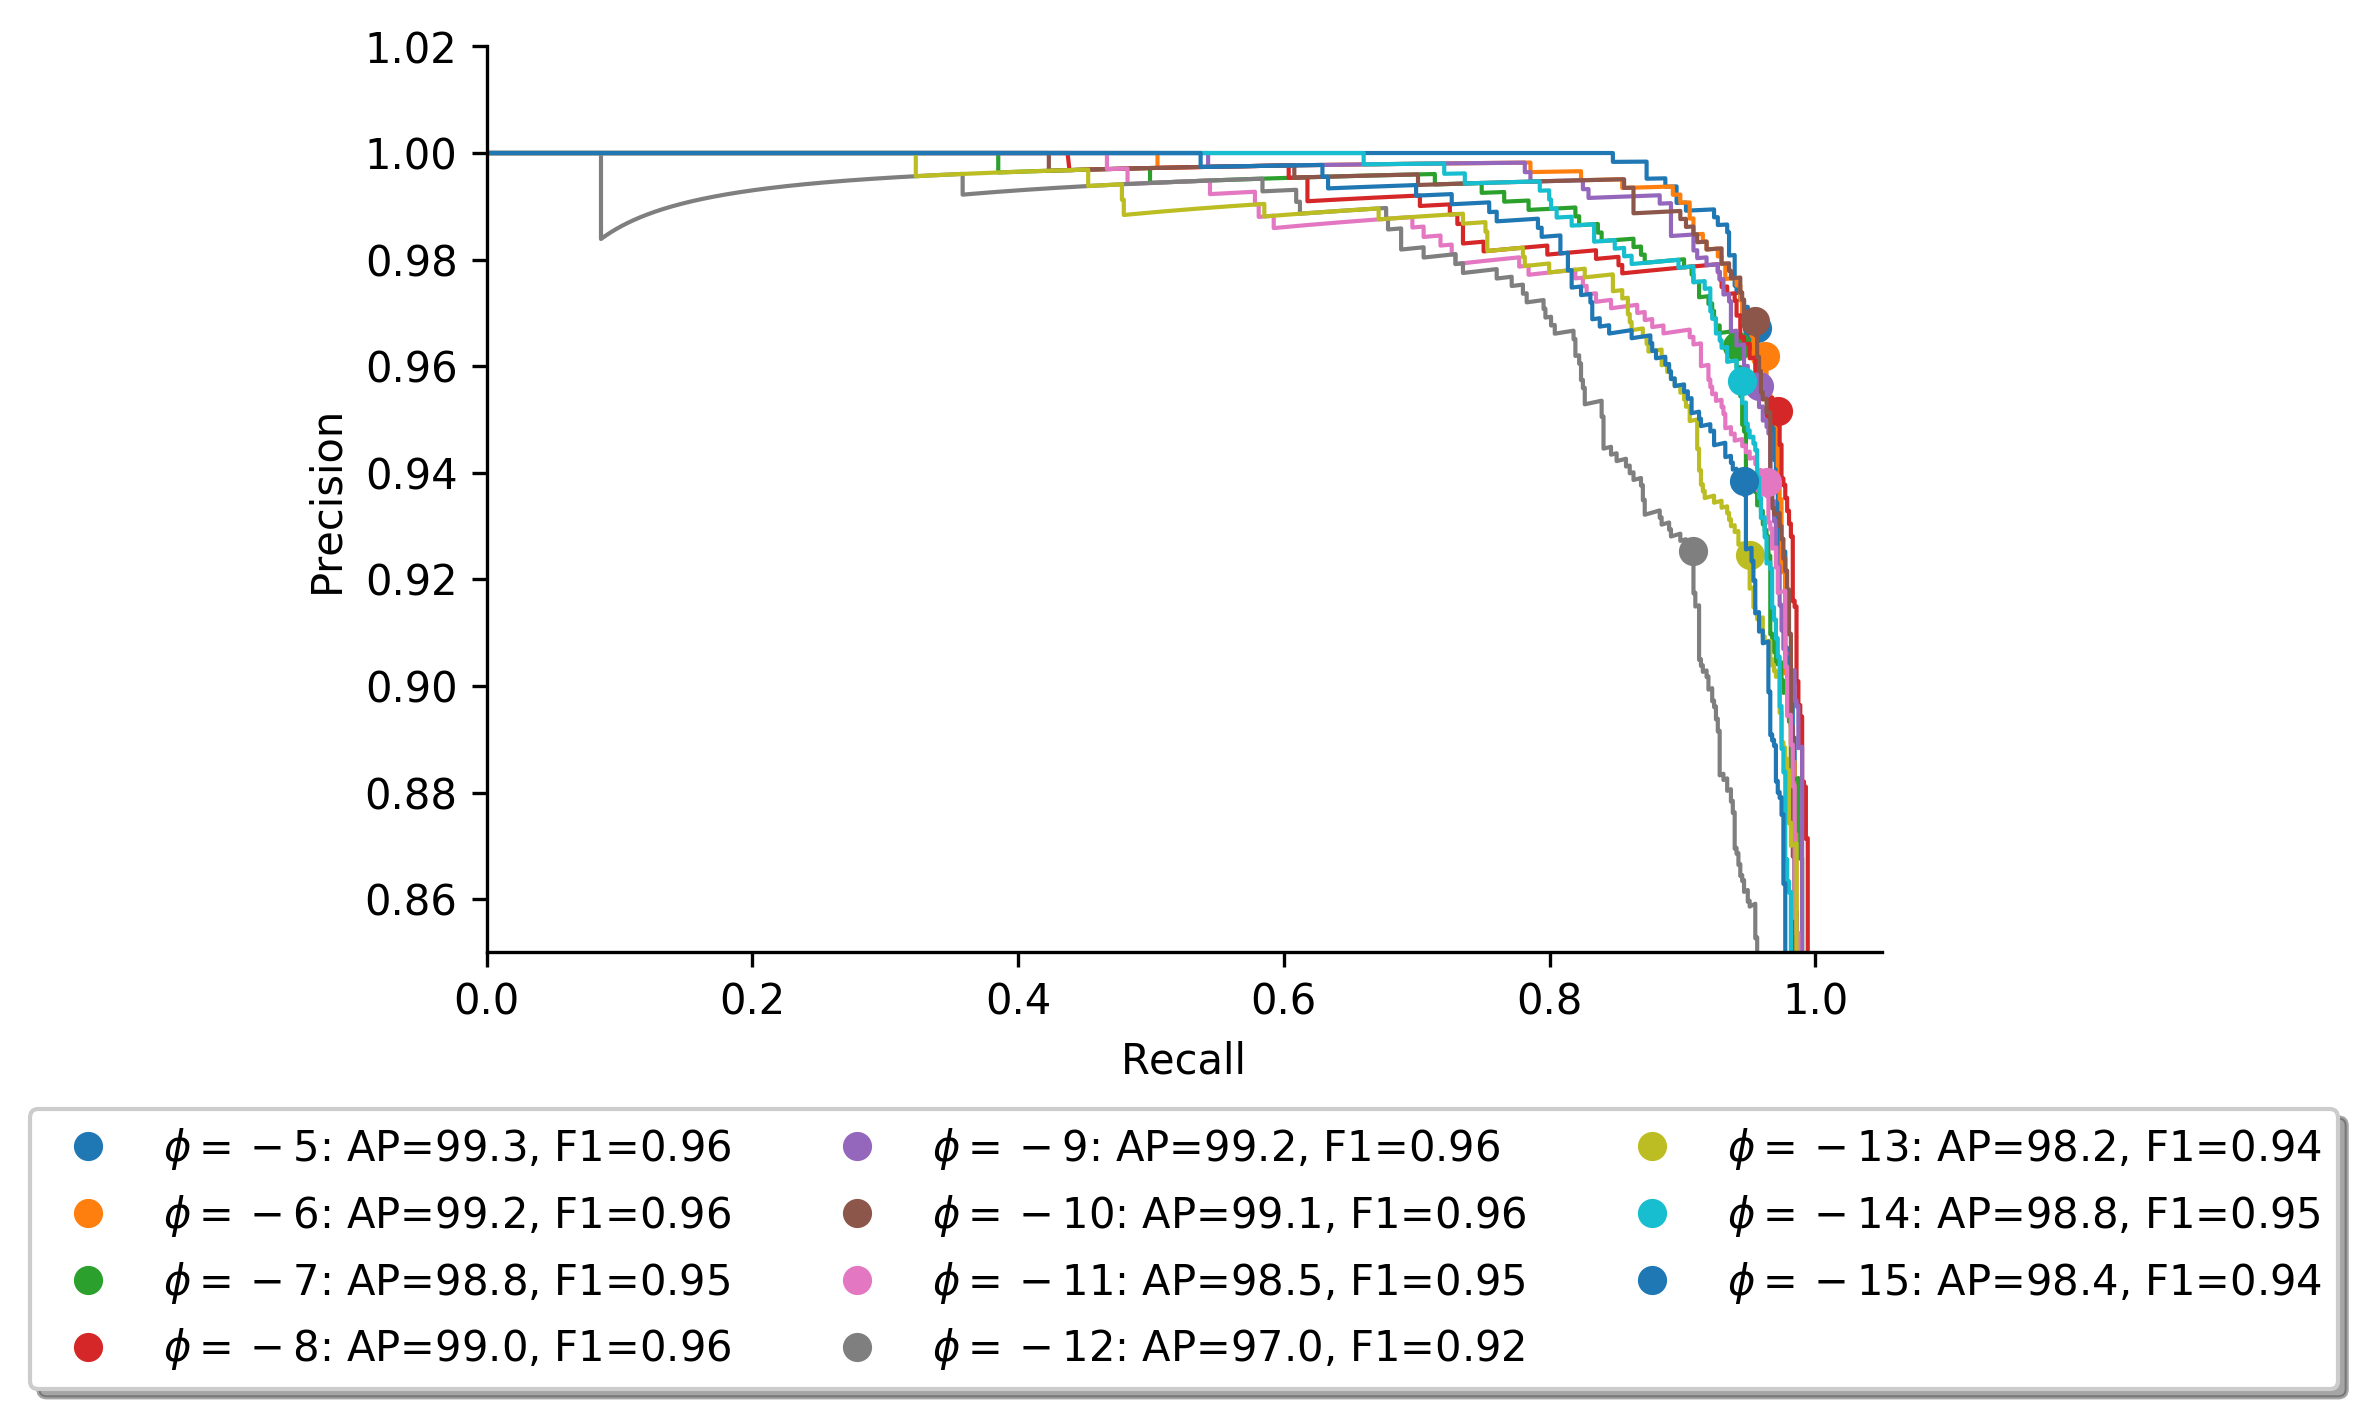
\includegraphics[width=0.95\textwidth]{figures/chapter_6/efn_scaled-pr_curve}
        \end{center}
        \caption{EFN Skalierung von $\phi=[-5,-15]$}
        \label{ch6:fig:efn_scale}
    \end{small}
\end{figure}

Das \SC{EFN-N15} erzielt bei einem Schwellwert von $0.665$ einen F1 Wert von $0.94$, welcher sich aus Precision und Recall von jeweils $0.94$ zusammensetzt.


\subsection*{Kombiniert}
Zuletzt wurde erneut ein Inferenztest mit beiden Komponenten ausgeführt.
Dabei wurden die Bilder mit dem Faktor $0.5$ herunterskaliert und anschließend die \acp{ROI} mit dem \SC{EFN-N15} klassifiziert.

Die Genauigkeit sank dabei nur marginal.
Jedoch ist ein signifikanter Geschwindigkeitsgewinn zu erkennen, sodass eine Mindest-Traktorgröße von rund $30 \times 30$ Pixel für zukünftige Aufnahmen angestrebt werden sollte (vgl. \autoref{ch6:tab:speed}).

\begin{figure}[H]
    \begin{small}
        \begin{center}
            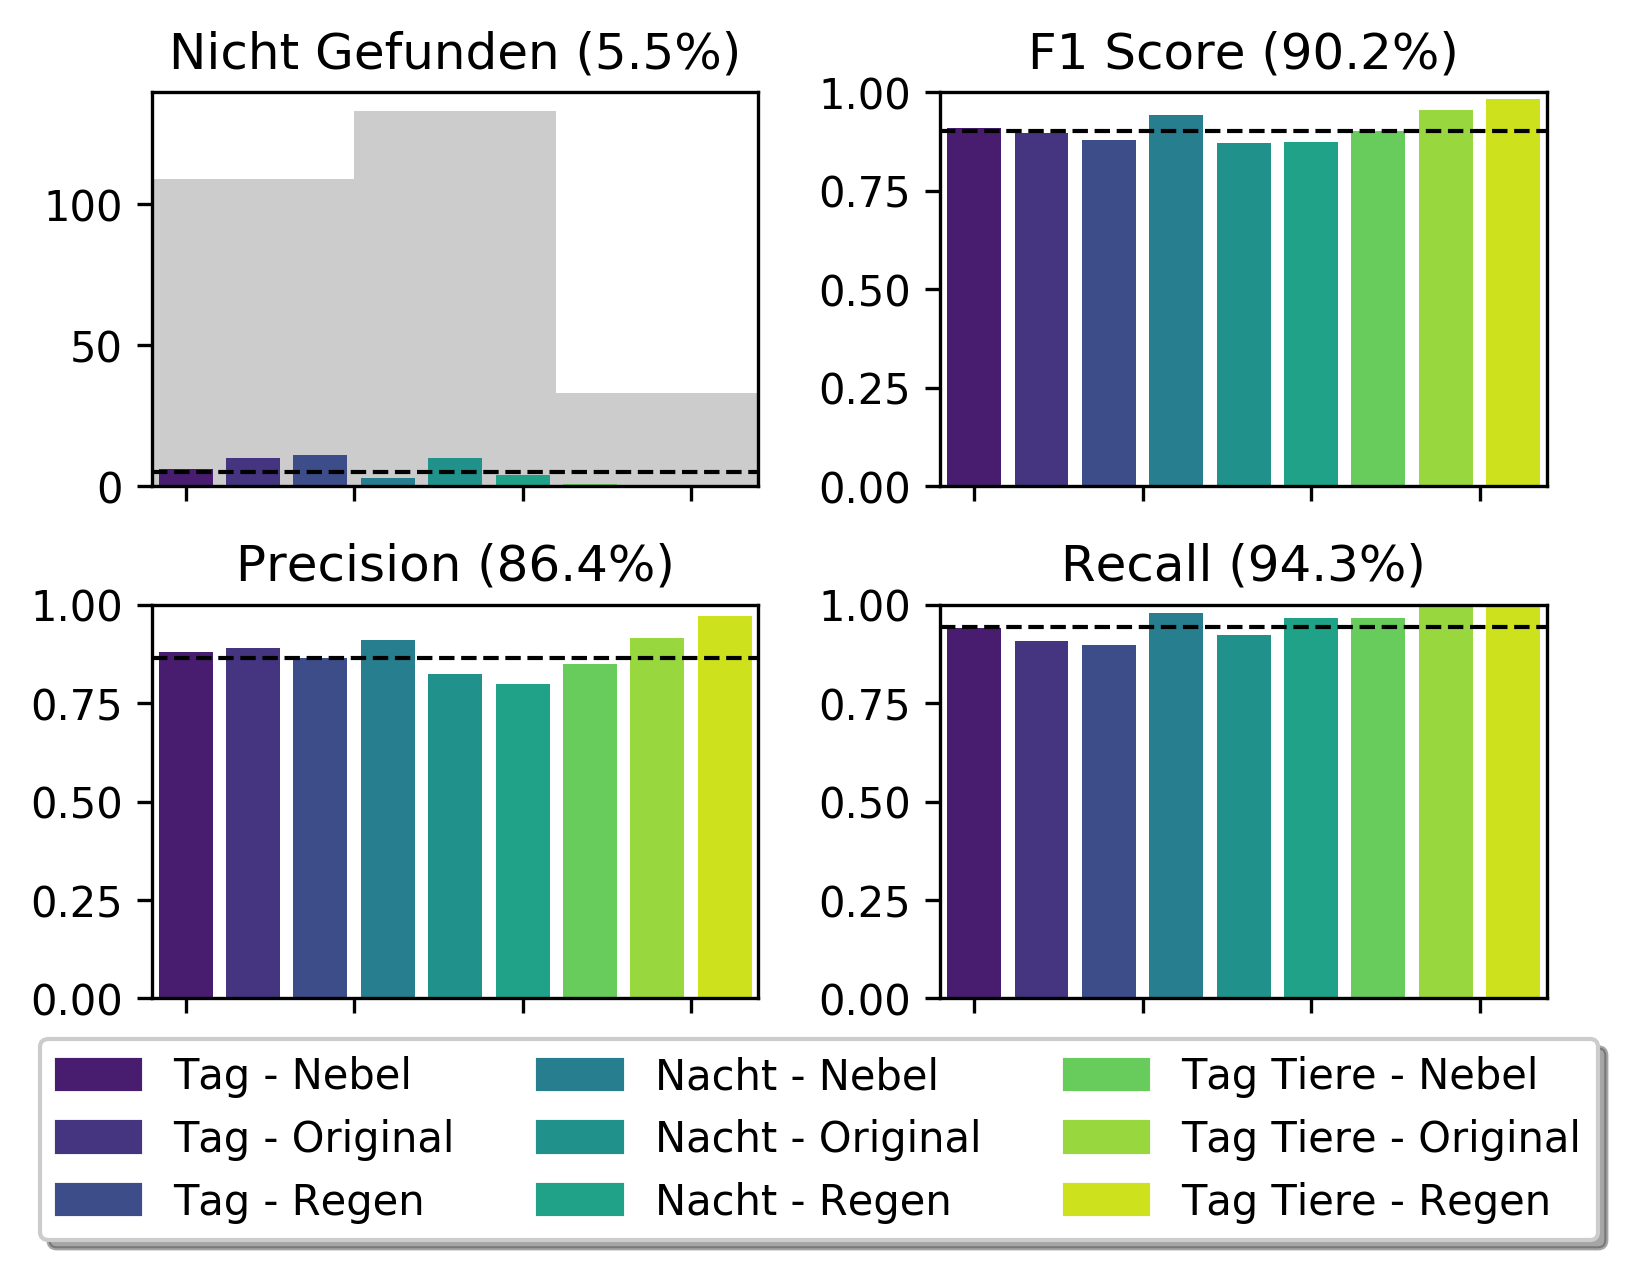
\includegraphics[width=0.95\textwidth]{figures/chapter_6/inference-scaled-metrics}
        \end{center}
        \caption[Skalierte Inferenzergebnisse]
            {Skalierte Inferenzergebnisse - Eingangsbild $0.5$ \& \SC{EFN-N15}}
        \label{ch6:fig:scale_metrics}
    \end{small}
\end{figure}

\begin{table}[H]
    \centering
    \begin{tabular}{cl|c}
    \textbf{} &
    \textbf{Skalierung} &
    \BF{Eingaben/Sekunde} \\ \shline

    \parbox[t]{2mm}{\multirow{3}{*}{\rotatebox[origin=c]{90}{1.0}}} &
      BMOG & 2.9 \\
    & \SC{EFN-N5} & 38 \\
    & \SC{EFN-N5 TRT} & 108 \\ \hline

    \parbox[t]{2mm}{\multirow{3}{*}{\rotatebox[origin=c]{90}{0.5}}} &
      BMOG & 10.3 \\
    & \SC{EFN-N15} & 106 \\
    & \SC{EFN-N15 TRT} & 1250 \\ \hline
    \end{tabular}
    \caption{Geschwindigkeit BMOG und EFN bei unterschiedlichen Skalierungen}
    \label{ch6:tab:speed}
\end{table}

Getestet wurde der Durchsatz der \acp{CNN} auf einer GPU der Serie \SC{RTX 2080 Ti}, der \ac{BGS} mit der CPU \SC{EPYC Rome} von \SC{AMD}.
Bei beiden Komponenten handelt es sich um leistungsstarke Workstation Hardware.
Deshalb sollten die Ergebnisse nicht direkt auf den realen Anwendungsfall übertragen werden, sie sind jedoch ein erster Indikator für die Laufzeit.

Für die \acp{CNN} wurden ebenfalls die mit \SC{TensorRT} (TRT) optimierten Netze getestet.
Diese erzielen eine enorme Geschwindigkeitkeitssteigerung.

\section{Diskussion der Ergebnisse} \label{ch6:discussion}
Im Folgenden werden die Anforderungen aus \autoref{ch4:requirements} und die Forschungsfragen aus \autoref{ch4:questions} betrachtet.

\bigskip
Funkionale Anforderungen:
\begin{itemize}
    \item Die Ergebnisse des Prototypen legen dar, dass mithilfe des Konzeptes in einem Radius von 300 Metern Traktoren gefunden und klassifiziert werden können.

    \item Dabei haben die simulierten Wettereinwirkungen Regen und Nebel keinen großen Einfluss.
    Für den realen Anwendungsfall gilt jedoch, dass die Linse der Kamera verregnet werden kann. 
    Das wurde in dieser Arbeit nicht getestet.

    \item Das Erkennen der Traktoren zu verschiedenen Tageszeit hat mit hoher Genauigkeit funktioniert.
    Jedoch werden dabei Großteils \IT{weiße Flecken} erkannt.
    Falls das für die reale Anwendung nicht ausreicht, sollte eine Nachtsichtkamera verwendet werden.

    \item Die Alarmgabe konnte aus Zeitgründen nicht evaluiert werden.
    Jedoch wurden zwei Ansätze dazu in \autoref{ch5:alarm} vorgestellt.
    Die Dauer für die Alarmgabe hängt dabei von der Traktorgeschwindigkeit ab, da für eine zuverlässige Vorhersage der Traktor aus möglichst vielen Winkeln aufgenommen werden sollte.
    In einem Beispiel wurde die dazu benötigte Zeit auf eine Minute geschätzt und erfüllt daher die Fünfminutengrenze.
    Ebenfalls hat sich gezeigt, dass eine Fehlklassifikation für mehrere Bilder unwahrscheinlich ist, sodass ein Alarm auch schon schneller gegeben werden könnte.
    Für die skalierte Variante ergibt sich eine Wahrscheinlichkeit von $0.136^{Anzahl}$ (inverse Precision).
    Bei drei Positiv-Vorhersagen liegt die Wahrscheinlichkeit für einen Fehlalarm folglich mit $0.136^3 = 0.0025$ unter einem Prozent.
\end{itemize}

Nicht-funktionale Anforderungen:
\begin{itemize}
    \item Die nicht-funktionalen Anforderungen wurden ebenfalls weitestgehend erfüllt.
    Die Komponenten wunrden in Python entwickelt und können einfach ausgetauscht werden.
    Es können somit verschiedene \acp{CNN} und \acp{BGS} zum Einsatz kommen.

    \item Die tatsächliche Stromkosten wurden nicht bestimmt.
    Es ist allerdings davon auszugehen, dass diese relativ niedrig sind, da für das Erkennen von Traktoren keine hohe Bildwiederholungsrate benötigt wird.
\end{itemize}

Forschungsfragen:
\begin{itemize}
    \item Traktoren des Prototypen konnten mit dem Konzept bestehend aus \ac{BGS} und \ac{CNN} zuverlässig erkannt werden.
    \item \IT{Wie schnell können Traktoren sinnvoll erkannt werden?}
    Siehe funktionale Anforderungen Punkt 4.
    \item Für die Mindestgröße der Traktoren im Bild wurde eine Pixelgröße von rund $30 \times 30$ bestimmt. 
\end{itemize}